\documentclass{article}
\usepackage[T1]{fontenc}
\usepackage{lmodern}
\usepackage{graphicx}
\usepackage{amsmath,amssymb}
\usepackage[a4paper,margin=2cm]{geometry}
\usepackage[absolute,overlay]{textpos}
\setlength{\TPHorizModule}{1mm}
\setlength{\TPVertModule}{1mm}
\usepackage[indonesian]{babel}
\usepackage{hyperref}
\setlength{\emergencystretch}{2em}
\title{07-Kripto-modern-dan-stream-cipher-2026}
\author{pdf\_ppt\_to\_latex}
\date{}

\begin{document}

% --- unit llm 1 ---
% === Halaman 1 (llm) ===

\begin{center}
{\huge IF4020 kriptografi} \\
\vspace{10mm}
{\Huge \textcolor{red}{07-- Kriptografi Modern dan Stream Cipher}} \\
\vspace{20mm}
\textbf{Oleh: Rinaldi M} \\
\vspace{10mm}
Program Studi Teknik Informatika \\
Sekolah Teknik Elektro dan Informatika \\
Institut Teknologi Bandung \\
2026
\end{center}

\newpage

% --- unit llm 2 ---
% === Halaman 2 (llm) ===

\section*{Pendahuluan}

\begin{itemize}
    \item Kriptografi modern adalah era kriptografi setelah penemuan komputer digital (awal tahun 1970-an).
    \item Perkembangan teknologi komputer digital membuat hampir semua bidang ilmu pengetahuan berkembang pesat, termasuk kriptografi.
    \item Komputer digital merepresentasikan data dan informasi dalam biner.
    \item Algoritma kriptografi modern beroperasi dalam mode bit (bandingkan dengan algoritma kriptografi klasik beroperasi dalam mode karakter)
    \begin{itemize}
        \item kunci, plainteks, cipherteks, diproses dalam rangkaian bit
        \item operasi \textbf{xor} paling banyak digunakan di dalam algoritmanya
    \end{itemize}
\end{itemize}

\newpage

% --- unit llm 3 ---
% === Halaman 3 (llm) ===

\begin{itemize}
    \item Meskipun disebut kriptografi modern, namun algoritmanya tetap menggunakan dua teknik dasar dasar di dalam kriptografi klasik: \textbf{teknik substitusi} dan \textbf{teknik transposisi (permutasi)},
    \item tetapi operasinya dibuat lebih kompleks, tidak sesederhana \textit{cipher} klasik. Tujuannya: agar \textit{cipher} modern lebih sulit dikriptanalisis
    \item Selain kedua teknik dasar tersebut, juga digunakan teknik lain seperti rotasi, kompresi, ekspansi, penjumlahan modulo, dan lain-lain.
    \item Kriptografi modern melahirkan konsep-konsep baru seperti algoritma kriptografi kunci-publik, fungsi \textit{hash}, protokol kriptografi, tanda-tangan digital, pembangkit bilangan acak, skema pembagian kunci, dsb.
\end{itemize}

\newpage

% --- unit llm 4 ---
% === Halaman 4 (llm) ===

\vspace{219.78mm}

\begin{center}
\Huge Diagram Blok Kriptografi Modern
\end{center}

\vspace{10mm}

% deskripsi: Diagram blok kriptografi modern yang menunjukkan hubungan hierarkis antara protokol jaringan aman (Secure Network Protocols), tujuan keamanan (Confidentiality, Data Integrity, Authentication, Non-Repudiation), mekanisme implementasi (Encryption, MACs/MICs, Challenge Responses, Digital Signatures), metode kriptografi (Symmetric Key Cryptography, Message Digest, Public Key Cryptography), dan komponen dasar (Block Cipher, Stream Cipher, Hash Function, Pseudo Random, Random Source, Elliptic Curve, DH RSA).
% bbox normalisasi: [0.1800, 0.1700, 0.8200, 0.9100]
\begin{textblock*}{134.40mm}(37.80mm,50.49mm)
\noindent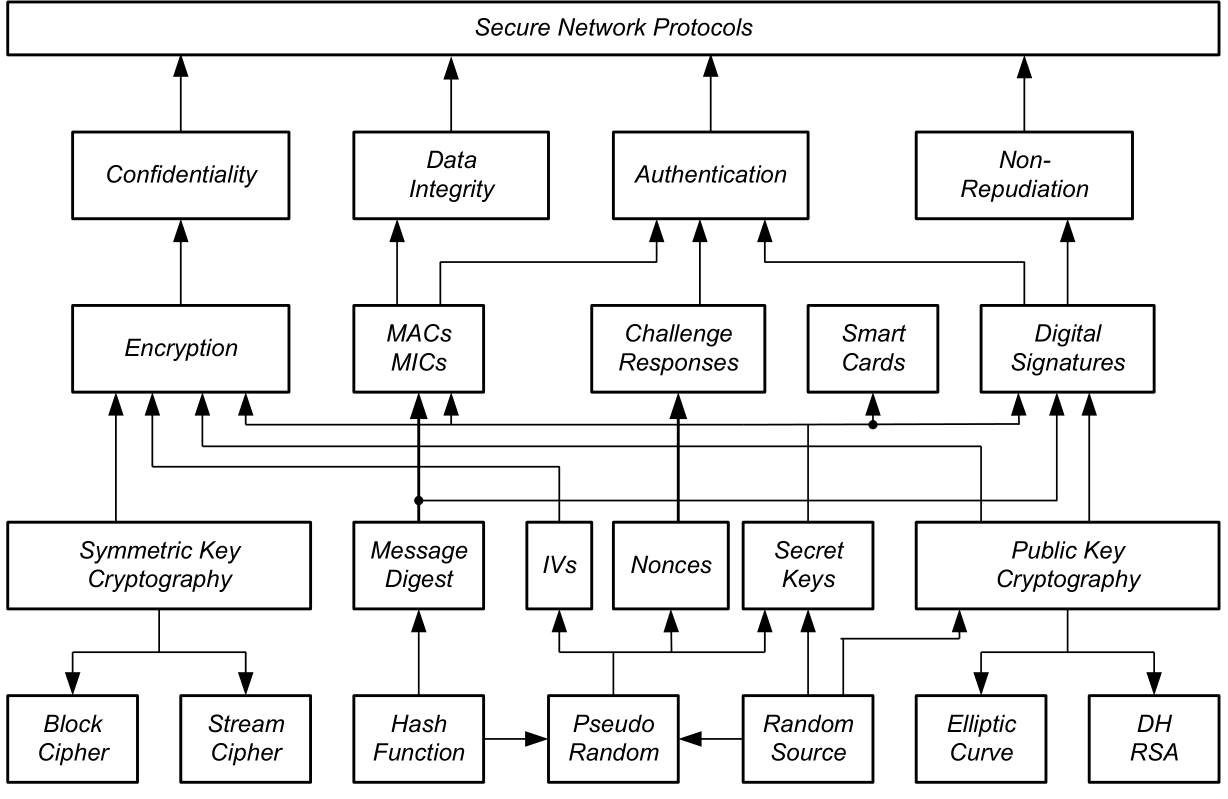
\includegraphics[width=134.40mm,height=219.78mm]{images/llm/page_004_img_01.png}%
\end{textblock*}

\newpage

% --- unit llm 5 ---
% === Halaman 5 (llm) ===

\section*{Bit, Byte, dan Kode Heksadesimal}

\vspace{68.31mm}

\begin{itemize}
    \item Pesan di dalam \textit{cipher} modern dienkripsi bit-per-bit atau \textit{byte-per-byte}, atau dalam kelompok bit (\textit{byte}).
    \[ 1\text{ byte} = 8\text{ bit} \]
    \item Pada beberapa algoritma kriptografi, pesan dikodekan ke dalam kode heksadesimal (\textbf{Hex}).
    \[ 1\text{ kode hex} = 4\text{ bit} \]
    \vspace{5mm}
    \item Contoh: Pesan $\text{1001110101101010}$ dalam kode Hex dengan cara membagi pesan menjadi blok 4-bit:
    \[ \text{1001 1101 0110 1010 = 9D6A} \]
\end{itemize}

% deskripsi: Tabel konversi biner 4-bit ke kode heksadesimal
% bbox normalisasi: [0.1300, 0.4800, 0.6700, 0.7100]
\begin{textblock*}{113.40mm}(27.30mm,142.56mm)
\noindent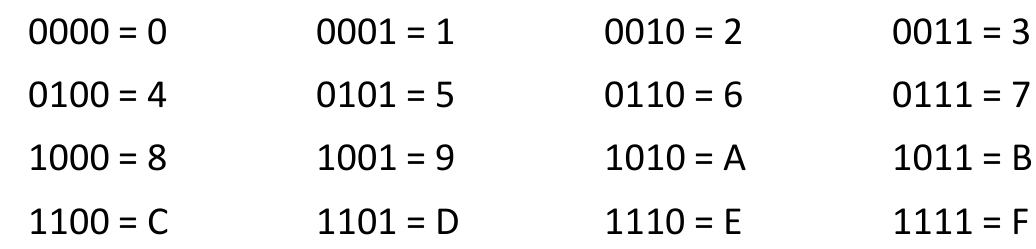
\includegraphics[width=113.40mm,height=68.31mm]{images/llm/page_005_img_01.png}%
\end{textblock*}

\newpage

% --- unit llm 6 ---
% === Halaman 6 (llm) ===

\vspace{225.72mm}

\begin{itemize}
  \item Konversi teks ke biner: \url{https://www.rapidtables.com/convert/number/string-to-binary.html}
\end{itemize}
\vspace{10mm}

% deskripsi: Screenshot halaman web RapidTables yang menunjukkan alat konversi teks ke biner dengan input 'Halo' dan output binernya.
% bbox normalisasi: [0.0780, 0.1500, 0.5300, 0.9100]
\begin{textblock*}{94.92mm}(16.38mm,44.55mm)
\noindent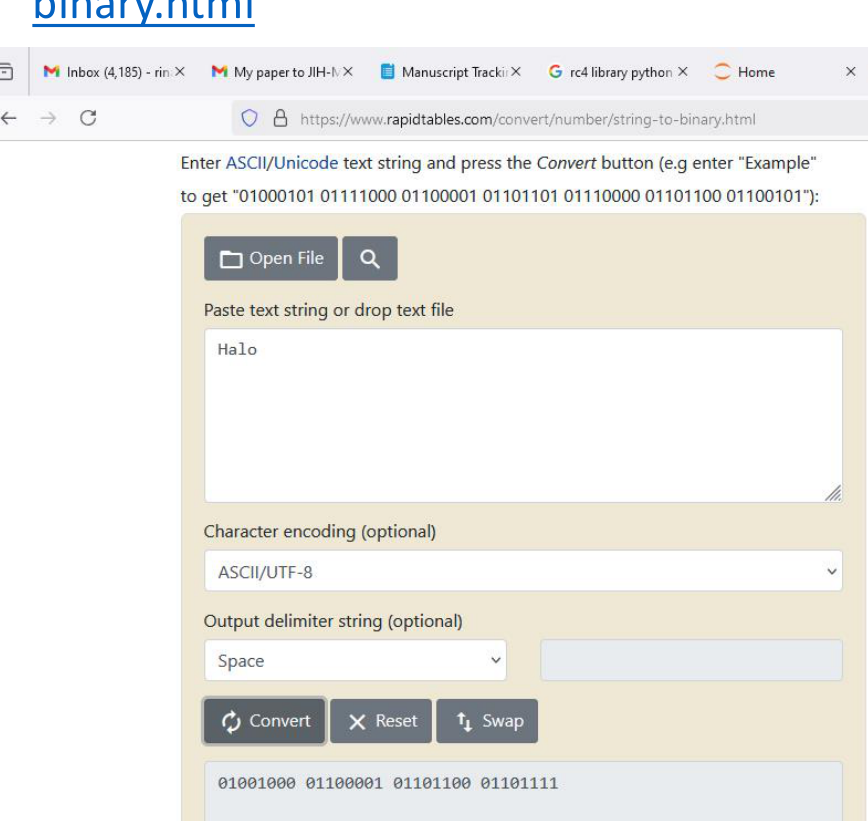
\includegraphics[width=94.92mm,height=225.72mm]{images/llm/page_006_img_01.png}%
\end{textblock*}

\newpage

% --- unit llm 7 ---
% === Halaman 7 (llm) ===

Contoh:\
\nHalo $\rightarrow$ 01001000 01100001 01101100 01101111\
\vspace{10mm}
Indonesia emas 2045 $\rightarrow$01001001 01101110 01100100 01101111 01101110\
01100101 01110011 01101001 01100001 00100000 01100101 01101101\
01100001 01110011 00100000 00110010 00110000 00110100 00110101

\newpage

% --- unit llm 8 ---
% === Halaman 8 (llm) ===

\vspace{246.51mm}

Konversi biner ke hex:

% deskripsi: Screenshot alat konversi biner ke heksadesimal dari situs RapidTables yang menunjukkan konversi bilangan biner 110101010111000101 menjadi heksadesimal D5C5 dan desimal 54725.
% bbox normalisasi: [0.0700, 0.1100, 0.9400, 0.9400]
\begin{textblock*}{182.70mm}(14.70mm,32.67mm)
\noindent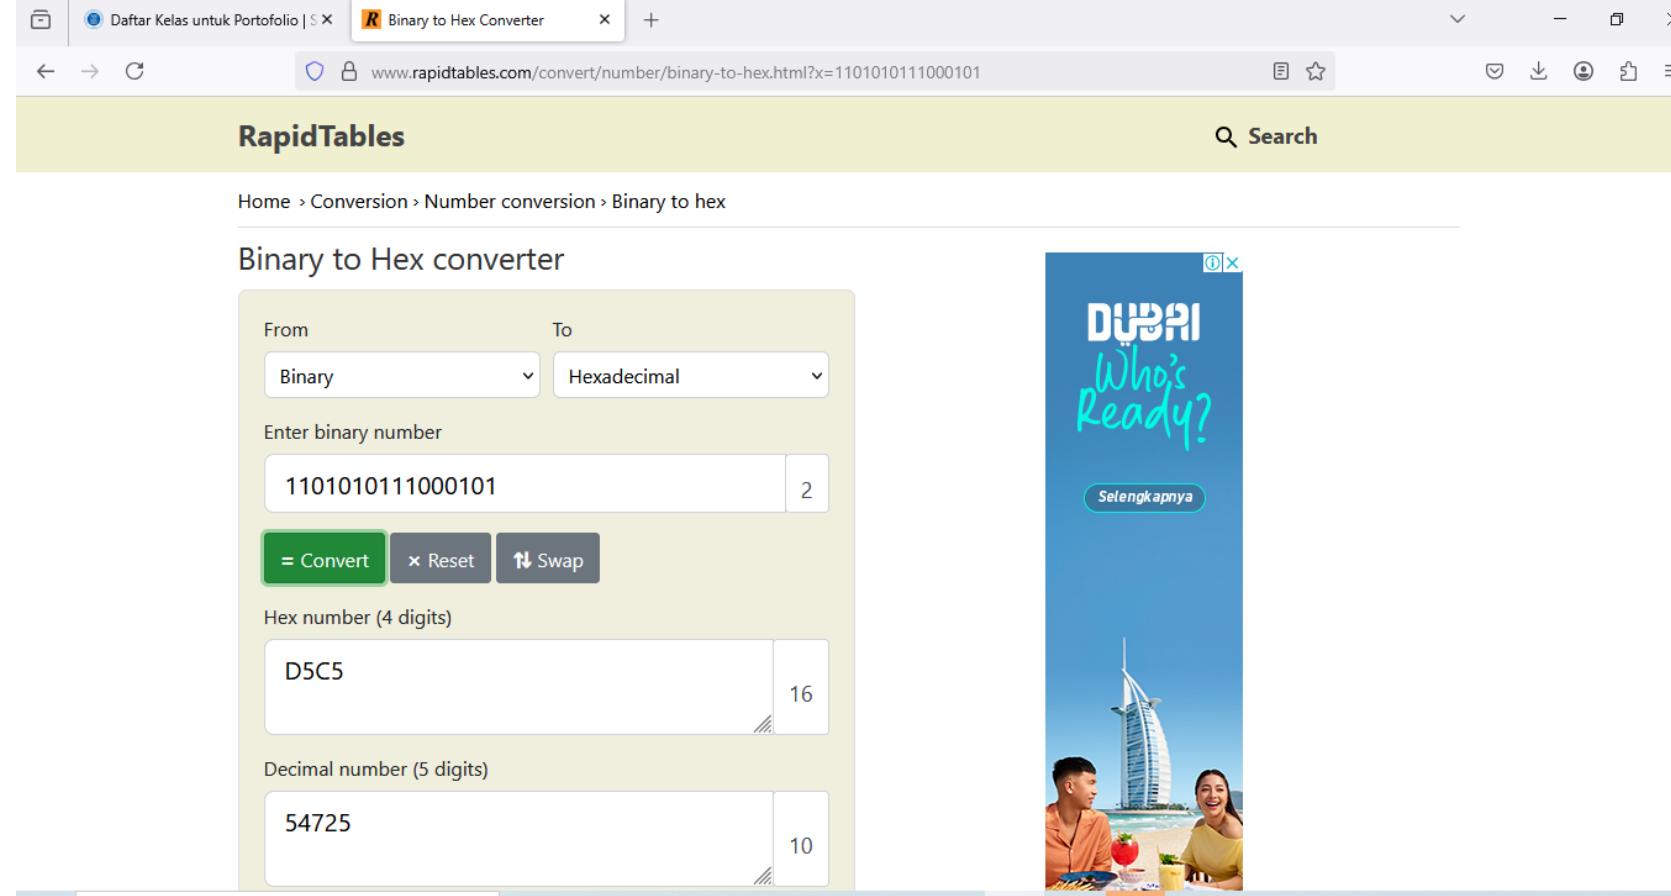
\includegraphics[width=182.70mm,height=246.51mm]{images/llm/page_008_img_01.png}%
\end{textblock*}

\newpage

% --- unit llm 9 ---
% === Halaman 9 (llm) ===

\section*{Operasi XOR}

\begin{itemize}
    \item Di dalam \textit{cipher} modern, operasi XOR adalah operasi yang paling sering digunakan
    \item Notasi: $\oplus$
    \item Operasi:
    \[
    \begin{aligned}
    0 \oplus 0 &= 0 & 0 \oplus 1 &= 1 \\
    1 \oplus 0 &= 1 & 1 \oplus 1 &= 0
    \end{aligned}
    \]
\end{itemize}

\vspace{10mm}

% deskripsi: Tabel kebenaran untuk operasi XOR dengan kolom a, b, dan hasil a XOR b.
% bbox normalisasi: [0.1920, 0.6280, 0.4380, 0.9150]
\begin{textblock*}{51.66mm}(40.32mm,186.52mm)
\noindent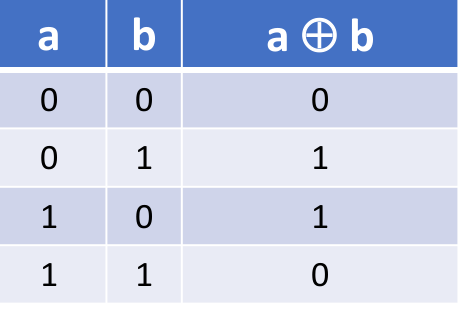
\includegraphics[width=51.66mm,height=85.24mm]{images/llm/page_009_img_01.png}%
\end{textblock*}

\newpage

% --- unit llm 10 ---
% === Halaman 10 (llm) ===

\begin{itemize}
    \item Sifat-sifat operasi XOR:
    \begin{enumerate}[(i)]
        \item $a \oplus a = 0$
        \item $a \oplus b = b \oplus a$
        \item $a \oplus (b \oplus c) = (a \oplus b) \oplus c$
    \end{enumerate}
\end{itemize}

Contoh:
\begin{enumerate}[(i)]
    \item $1 \oplus 1 = 0$
    \item $1 \oplus 0 = 0 \oplus 1 = 1$
    \item $1 \oplus (0 \oplus 1) = (1 \oplus 0) \oplus 1 = 0$
\end{enumerate}

\newpage

% --- unit llm 11 ---
% === Halaman 11 (llm) ===

\section*{Operasi Bitwise XOR}

\begin{itemize}
    \item Jika dua rangkaian dioperasikan dengan $XOR$, maka operasinya dilakukan dengan meng-$XOR$-kan setiap bit yang berkoresponden dari kedua rangkaian bit tersebut.
\end{itemize}

Contoh: $10011 \oplus 11001 = 01010$

\vspace{63.85mm}

yang dalam hal ini, hasilnya diperoleh sebagai berikut:

\vspace{10mm}

% deskripsi: Proses perhitungan bitwise XOR secara vertikal antara dua deret biner 10011 dan 11001 yang menghasilkan 01010.
% bbox normalisasi: [0.3160, 0.6570, 0.6960, 0.8720]
\begin{textblock*}{79.80mm}(66.36mm,195.13mm)
\noindent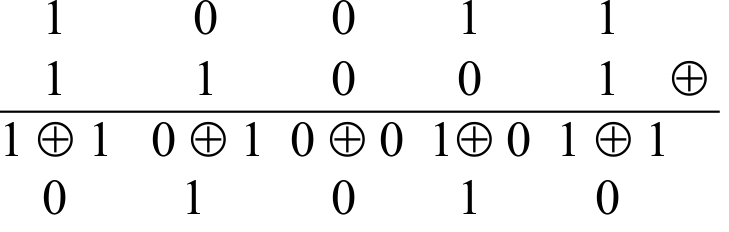
\includegraphics[width=79.80mm,height=63.85mm]{images/llm/page_011_img_01.png}%
\end{textblock*}

\newpage

% --- unit llm 12 ---
% === Halaman 12 (llm) ===

\section*{Cipher Sederhana dengan operasi XOR}

\begin{itemize}
    \item Sama seperti \textit{Vigenere Cipher}, tetapi dalam mode bit
    \item Setiap bit plainteks di-XOR-kan dengan setiap bit kunci.
\end{itemize}

\[ \text{Enkripsi: } C = P \oplus K \]
\[ \text{Dekripsi: } P = C \oplus K \]

\vspace{5mm}

Contoh:
\begin{tabular}{lll}
plainteks & 01100101 & (karakter 'e') \\
kunci & 00110101 $\oplus$ & (karakter '5') \\
\hline
cipherteks & 01010000 & (karakter 'P') \\
kunci & 00110101 $\oplus$ & (karakter '5') \\
\hline
plainteks & 01100101 & (karakter 'e')
\end{tabular}

\newpage

% --- unit llm 13 ---
% === Halaman 13 (llm) ===

\begin{itemize}
    \item Jika panjang bit-bit kunci lebih pendek daripada panjang bit-bit pesan, maka bit-bit kunci diulang penggunaannya secara periodik (seperti halnya pada Vigenere Cipher)
    \item Contoh:
    \begin{align*}
    \text{Plainteks} & : 10010010101110101010001110001 \\
    \text{Kunci} & : 11011011011011011011011011011 \\
    \text{Cipherteks} & : 01001001110101110001010101010
    \end{align*}
\end{itemize}

\newpage

% --- unit llm 14 ---
% === Halaman 14 (llm) ===

\vspace{184.14mm}

Program C++ untuk enkripsi-dekripsi file dengan cipher XOR sederhana

\vspace{10mm}

% deskripsi: Screenshot kode program C++ untuk enkripsi (enkrip_xor.cpp) dan dekripsi (dekrip_xor.cpp) menggunakan algoritma XOR sederhana.
% bbox normalisasi: [0.3500, 0.0000, 0.9700, 0.6200]
\begin{textblock*}{130.20mm}(73.50mm,0.00mm)
\noindent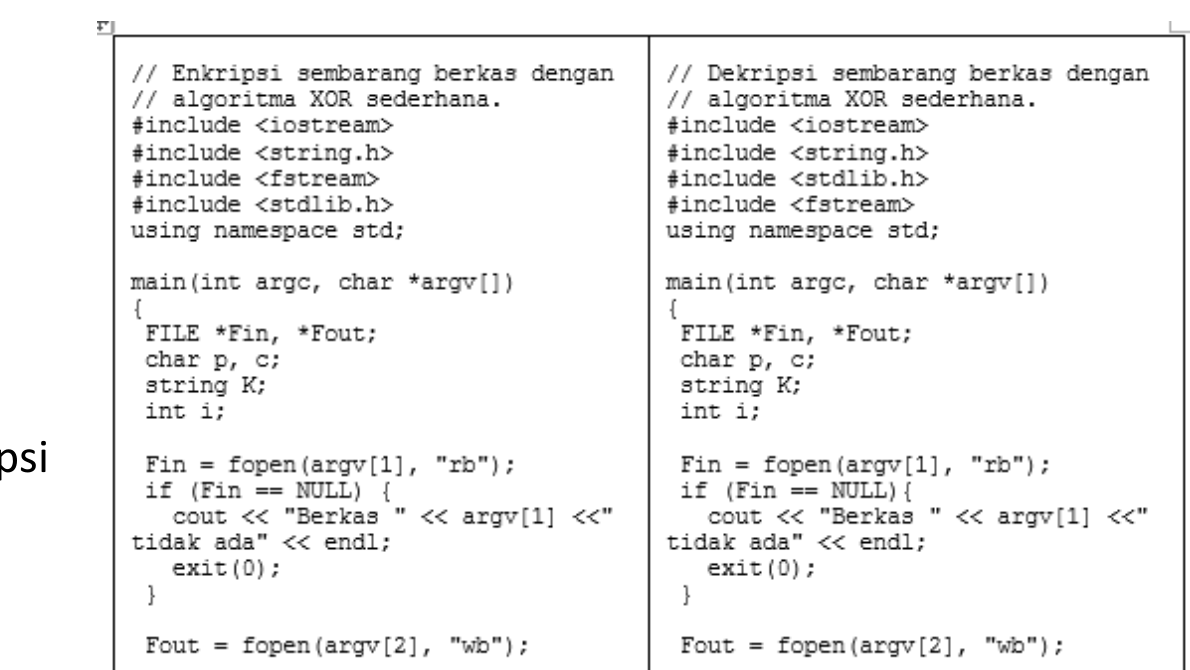
\includegraphics[width=130.20mm,height=184.14mm]{images/llm/page_014_img_01.png}%
\end{textblock*}

\newpage

% --- unit llm 15 ---
% === Halaman 15 (llm) ===

% (tidak ada teks dari model)

% deskripsi: Screenshot Command Prompt yang menunjukkan proses enkripsi dan dekripsi file teks menggunakan program enkrip_xor dan dekrip_xor dengan kata kunci 'viruscorona'.
% bbox normalisasi: [0.0650, 0.2010, 0.9350, 0.8140]
\begin{textblock*}{182.70mm}(13.65mm,59.70mm)
\noindent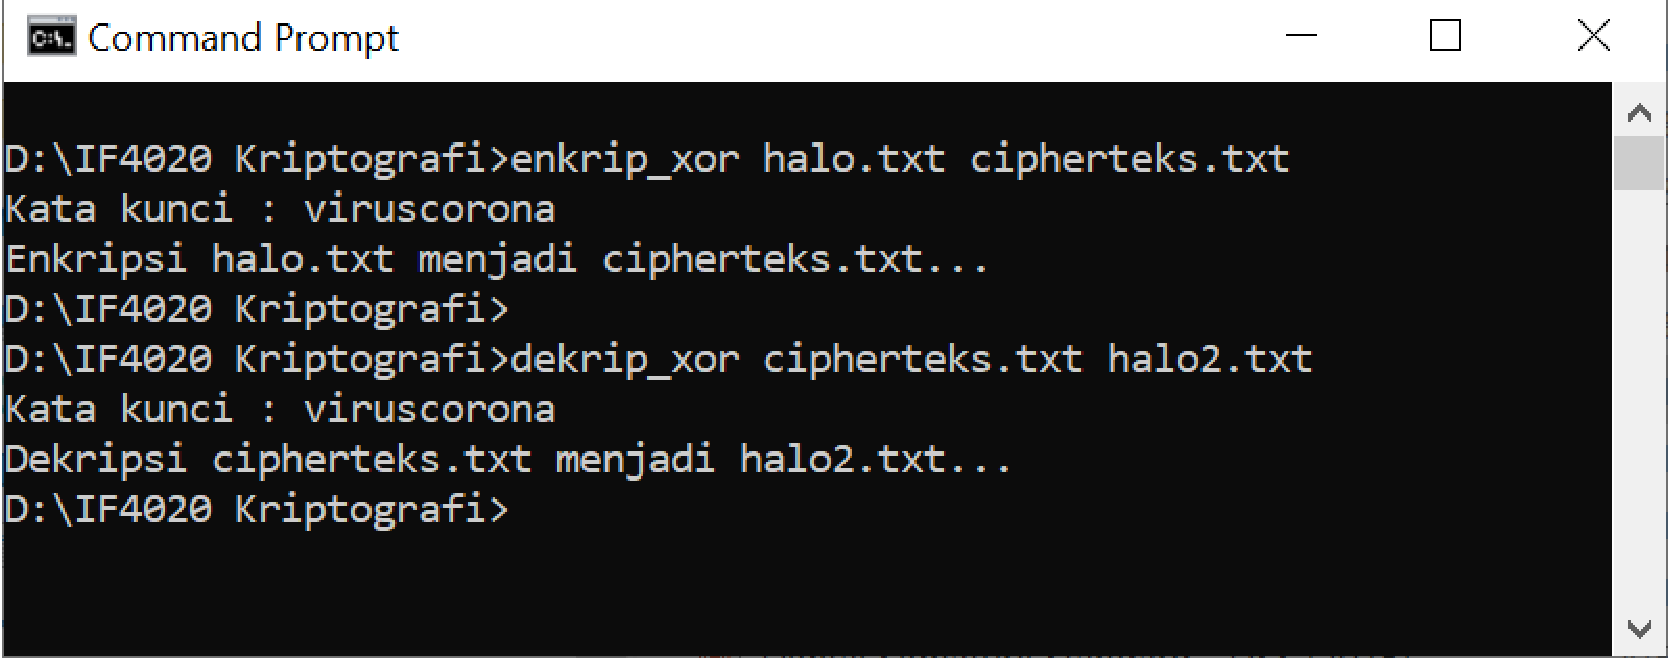
\includegraphics[width=182.70mm,height=182.06mm]{images/llm/page_015_img_01.png}%
\end{textblock*}

\newpage

% --- unit llm 16 ---
% === Halaman 16 (llm) ===

\vspace{175.23mm}

\section*{Program Python untuk enkripsi-dekripsi file dengan cipher XOR sederhana}

\vspace{10mm}

% deskripsi: Screenshot kode program Python untuk fungsi xor_cipher_encrypt
% bbox normalisasi: [0.0100, 0.2200, 0.5000, 0.8100]
\begin{textblock*}{102.90mm}(2.10mm,65.34mm)
\noindent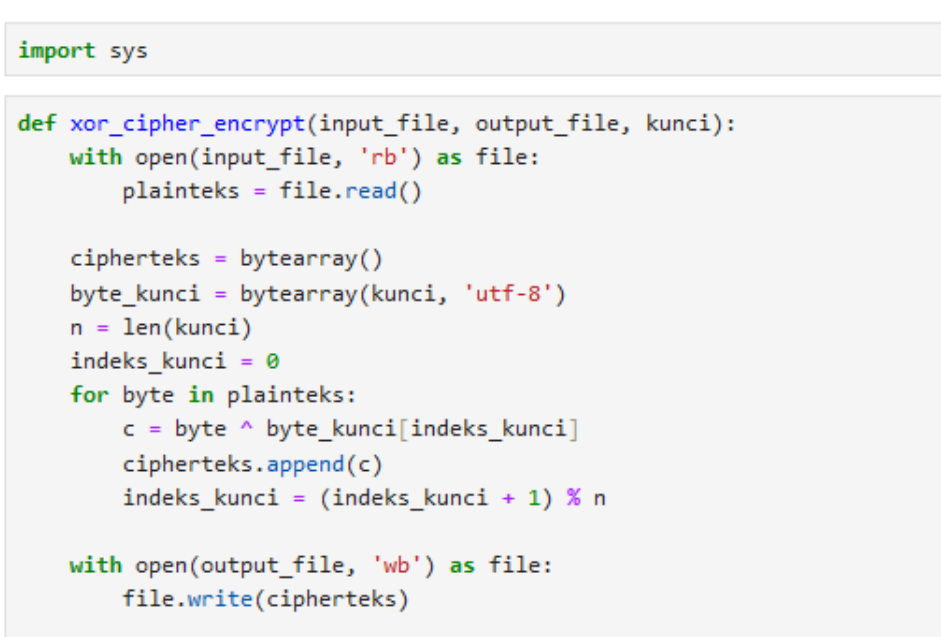
\includegraphics[width=102.90mm,height=175.23mm]{images/llm/page_016_img_01.png}%
\end{textblock*}

% deskripsi: Screenshot kode program Python untuk fungsi xor_cipher_decrypt
% bbox normalisasi: [0.5100, 0.2200, 0.9900, 0.8100]
\begin{textblock*}{100.80mm}(107.10mm,65.34mm)
\noindent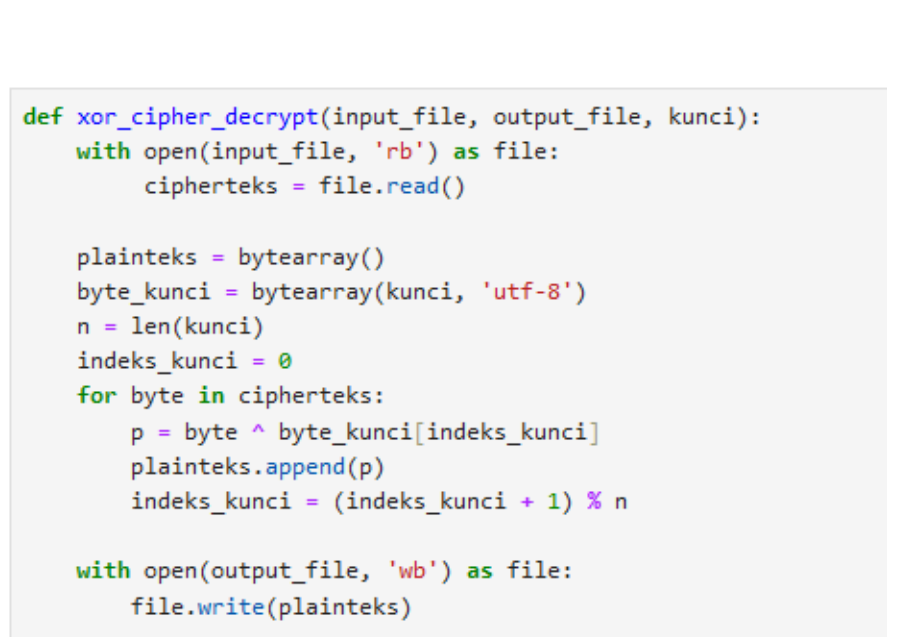
\includegraphics[width=100.80mm,height=175.23mm]{images/llm/page_016_img_02.png}%
\end{textblock*}

\newpage

% --- unit llm 17 ---
% === Halaman 17 (llm) ===

\vspace{216.81mm}

Contoh penggunaan:

% deskripsi: Screenshot cuplikan kode Python yang menunjukkan contoh penggunaan fungsi xor_cipher_encrypt dan xor_cipher_decrypt, lengkap dengan input pengguna untuk nama file plaintext, ciphertex, dan kata kunci.
% bbox normalisasi: [0.1070, 0.2010, 0.7220, 0.9310]
\begin{textblock*}{129.15mm}(22.47mm,59.70mm)
\noindent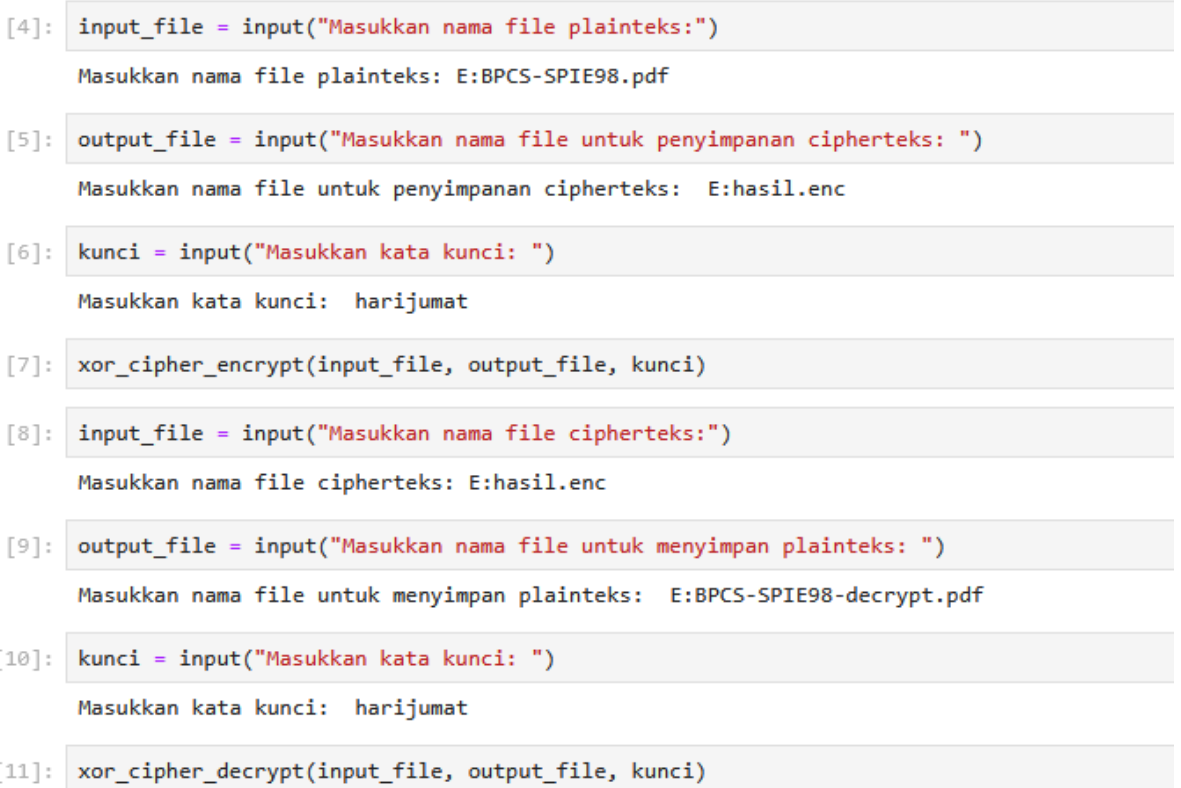
\includegraphics[width=129.15mm,height=216.81mm]{images/llm/page_017_img_01.png}%
\end{textblock*}

\newpage

% --- unit llm 18 ---
% === Halaman 18 (llm) ===

header for SPIE use

\begin{center}
\fbox{\begin{tabular}{c}
BPCS:Steganography Experimental Program site:\\ \url{http://www.datahide.org/BPCSe/QtechHV-program-e.html}
\end{tabular}}

\section*{Principle and applications of BPCS-Steganography}

Eiji Kawaguchi* \& Richard O. Eason**

* Kyushu Institute of Technology, Kitakyushu, Japan \\
** University of Maine, Orono, Maine 04469--5708

\subsection*{ABSTRACT}

Steganography is a technique to hide secret information in some other data (we call it a vessel) without leaving any apparent evidence of data alteration. All of the traditional steganographic techniques have limited information-hiding capacity. They can hide only 10\% (or less) of the data amounts of the vessel. This is because the principle of those techniques was either to replace a special part of the frequency components of the vessel image, or to replace all the least significant bits of a multi-valued image with the secret information stereotype.

Our new steganography uses an image as the vessel data, and we embed secret information in the bit-planes of the vessel. This technique makes use of the characteristics of the human vision system whereby a human cannot perceive any shape information in a very complicated binary pattern. We can replace all of the ``noise-like'' regions in the bit-planes of the vessel image with secret data without deteriorating the image quality. We termed our steganography ``BPCS-Steganography,'' which stands for Bit-Plane Complexity Segmentation Steganography.

We made an experimental system to investigate this technique in depth. The merits of BPCS-Steganography found by the experiments are as follows.

\begin{enumerate}
  \item T...
  \item A...
  \item C...
\end{enumerate}
\end{center}

\newpage

% --- unit llm 19 ---
% === Halaman 19 (llm) ===

\vspace{236.12mm}

Contoh hasil file cipherteks: hasil.enc

% deskripsi: Screenshot aplikasi Notepad yang menampilkan isi file 'hasil.enc' yang berisi teks acak hasil enkripsi (cipherteks).
% bbox normalisasi: [0.0640, 0.1250, 0.7720, 0.9200]
\begin{textblock*}{148.68mm}(13.44mm,37.12mm)
\noindent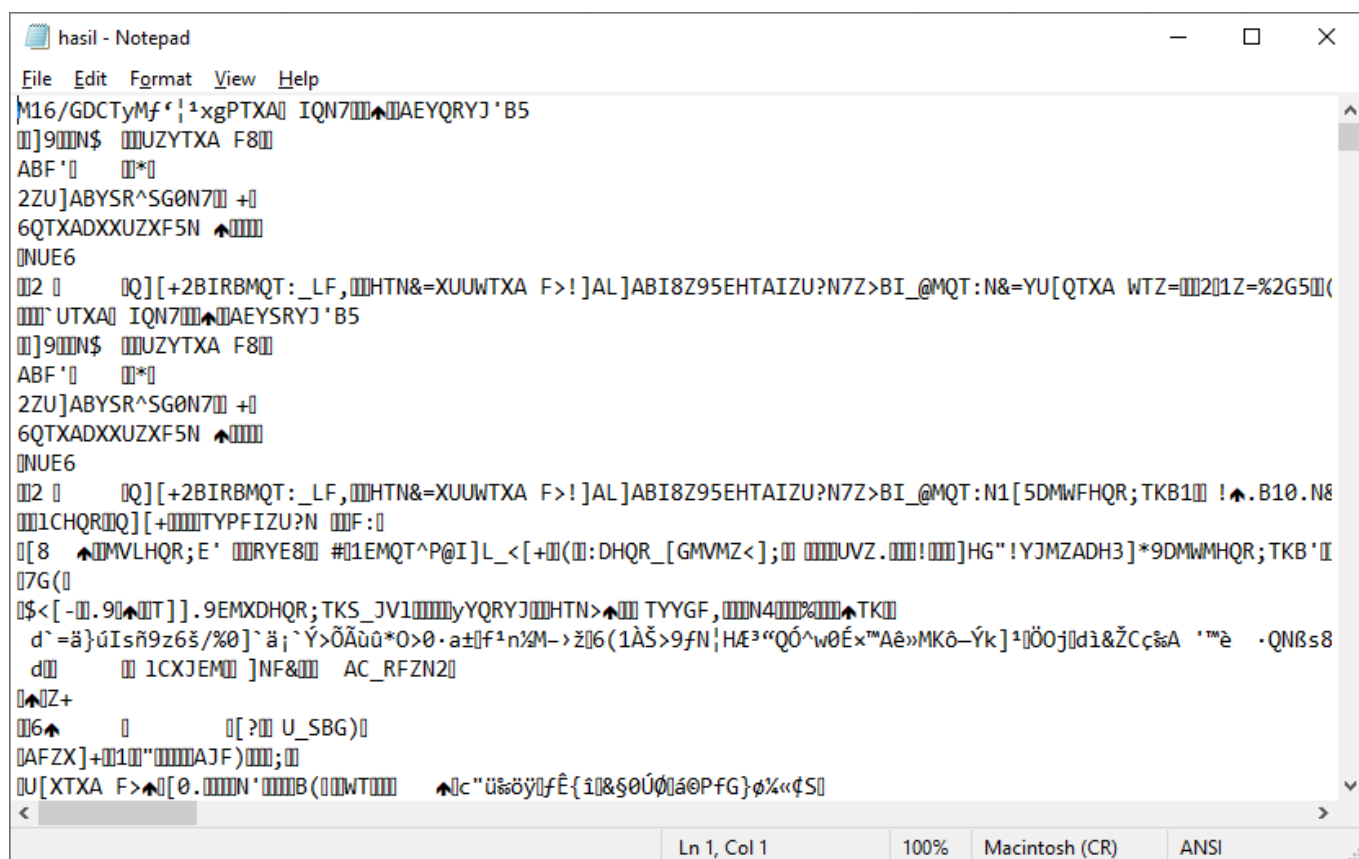
\includegraphics[width=148.68mm,height=236.12mm]{images/llm/page_019_img_01.png}%
\end{textblock*}

\newpage

% --- unit llm 20 ---
% === Halaman 20 (llm) ===

header for SPIE use

\begin{center}
\textbf{BPCS-Steganography Experimental Program site:}\
\url{http://www.datahide.org/BPCS e:QPtechHV-program-e.html}

\Large \textbf{Principle and applications of BPCS-Steganography}

\large Eiji Kawaguchi$^*$ and Richard O. Eason$^{**}$

\small $^*$ Kyushu Institute of Technology, Kitakyushu, Japan\
$^{**}$ University of Maine, Orono, Maine 04469-5708
\end{center}

\begin{center}
\textbf{ABSTRACT}
\end{center}

Steganography is a technique to hide secret information in some other data (we call it a \textit{vessel}) without leaving any apparent evidence of data alteration. All of the traditional steganographic techniques have limited information-hiding capacity. They can hide only $10\%$ (or less) of the data amounts of the vessel. This is because the principle of those techniques was either to replace a special part of the frequency components of the vessel image, or to replace all the least significant bits of a multi-valued image with the secret information.

Our new steganography uses an image as the vessel data, and we embed secret information in the bit-planes of the vessel. This technique makes use of the characteristics of the human vision system where by herself a human cannot perceive any shape information in a very complicated binary pattern. We can replace all of the ``noise-like'' regions in the bit-planes of the vessel image with secret data without deteriorating the image quality. We termed our steganography ``BPCS-Steganography,'' which stands for Bit-Plane Complexity Segmentation-steganography.

We made an experimental system to investigate this technique in depth. The merits of BPCS-Steganography found by the experiments are as follows.

\begin{enumerate}
    \item The information hiding capacity of a true color image is around $50\%$.
    \item A sharpening operation on the dummy image increases the embedding capacity quite a bit.
    \item Canonical Gray coded bit planes are more suitable for BPCS-Steganography than the standard binary bit planes.
\end{enumerate}

\newpage

% --- unit llm 21 ---
% === Halaman 21 (llm) ===

\begin{itemize}
  \item \textit{Cipher} XOR sederhana tidak aman, karena mudah dikriptanalisis dengan metode yang sama seperti metode Kasiski
\end{itemize}

\newpage

% --- unit llm 22 ---
% === Halaman 22 (llm) ===

\section*{Kategori \textit{cipher} berbasis bit}

\begin{enumerate}
    \item \textbf{Cipher Alir (\textit{Stream Cipher})}
    \begin{itemize}
        \item beroperasi pada bit (atau \textit{byte}) secara individual
        \item enkripsi/dekripsi pesan secara bit per bit (atau \textit{byte per byte}) hanya dengan operasi XOR saja
    \end{itemize}
    
    \item \textbf{Cipher Blok (\textit{Block Cipher})}
    \begin{itemize}
        \item beroperasi pada blok-blok bit (sekumpulan bit) \\ (contoh: 128-bit/blok = 16 byte/blok)
        \item enkripsi/dekripsi pesan secara blok per blok bit dengan komputasi yang lebih kompleks dan dilakukan berulang kali dalam sejumlah putaran.
    \end{itemize}
\end{enumerate}

\newpage

% --- unit llm 23 ---
% === Halaman 23 (llm) ===

% (tidak ada teks dari model)

% deskripsi: Diagram hierarki klasifikasi Kriptologi yang terbagi menjadi Kriptografi dan Kriptanalisis. Kriptografi selanjutnya terbagi menjadi Cipher Simetris, Cipher Asimetris, dan Fungsi Hash. Cipher Simetris terbagi lagi menjadi Block Ciphers dan Stream Ciphers.
% bbox normalisasi: [0.1100, 0.1700, 0.7800, 0.7500]
\begin{textblock*}{140.70mm}(23.10mm,50.49mm)
\noindent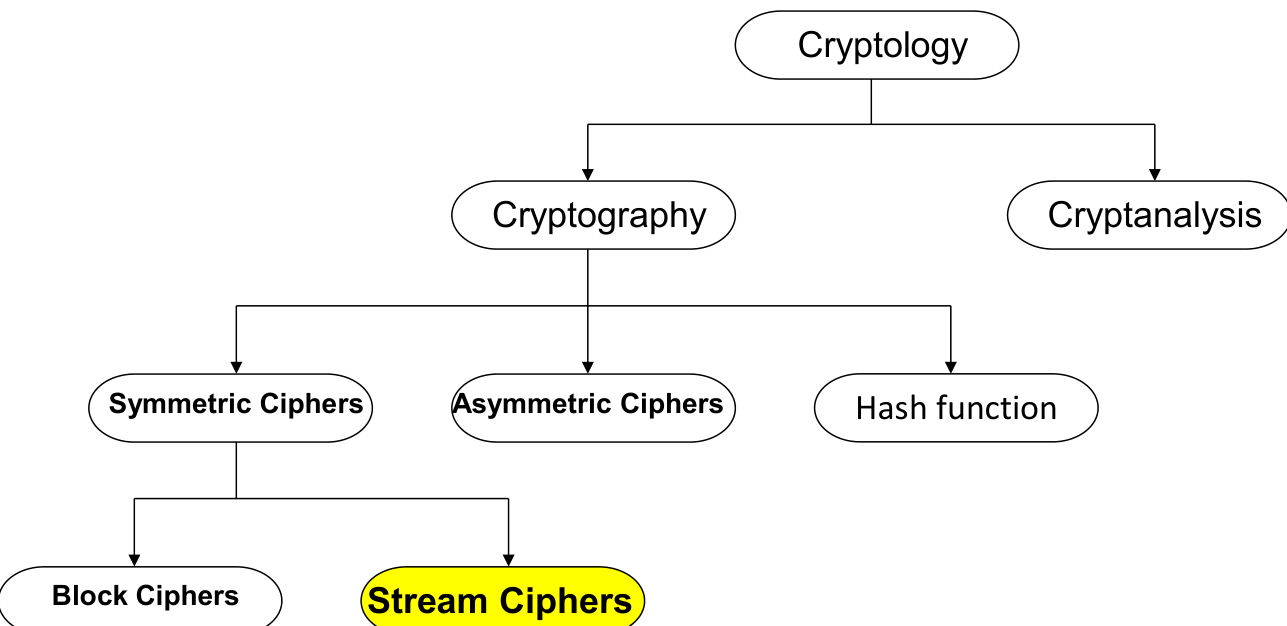
\includegraphics[width=140.70mm,height=172.26mm]{images/llm/page_023_img_01.png}%
\end{textblock*}

\newpage

% --- unit llm 24 ---
% === Halaman 24 (llm) ===

\section*{A. Stream Cipher}

\newpage

% --- unit llm 25 ---
% === Halaman 25 (llm) ===

\section*{Cipher Alir (Stream Cipher)}

\begin{itemize}
    \item Mengenkripsi plainteks menjadi chiperteks dengan cara:
    \begin{itemize}
        \item $1 \text{ bit plainteks} \oplus 1 \text{ bit kunci}$, atau
        \item $1 \text{ byte plainteks} \oplus 1 \text{ byte skunci}$, atau
        \item $n \text{ bit plainteks} \oplus n \text{ bit kunci}$
    \end{itemize}
    setiap kali enkripsi
    
    \item Dekripsi dilakukan dengan cara:
    \begin{itemize}
        \item $1 \text{ bit cipherteks} \oplus 1 \text{ bit kunci}$, atau
        \item $1 \text{ byte cipherteks} \oplus 1 \text{ byte skunci}$, atau
        \item $n \text{ bit cipherteks} \oplus n \text{ bit kunci}$
    \end{itemize}
    setiap kali dekripsi.
\end{itemize}

\newpage

% --- unit llm 26 ---
% === Halaman 26 (llm) ===

\vspace{121.77mm}

\section*{Diagram Umum \textit{Cipher} alir}

\vspace{60mm}

\begin{itemize}
    \item Bit-bit aliran kunci untuk enkripsi/dekripsi disebut \textit{keystream}
    \item \textit{Keystream} dibangkitkan oleh \textit{keystream generator} berdasarkan umpan (\textit{seed}) U.
    \item Enkripsi dan dekripsi dengan \textit{cipher} alir komputasinya sederhana dan cepat
    \item \textit{Keystream} $c_1, c_2, \dots$ di-XOR-kan dengan aliran bit-bit plainteks, $p_1, p_2, \dots$, menghasilkan aliran bit-bit cipherteks $c_1, c_2, \dots$:
    \[ c_i = p_i \oplus k_i \]
    \item Di sisi penerima dibangkitkan \textit{keystream} yang sama untuk mendekripsi aliran bit-bit cipherteks $c_1, c_2, \dots$ menjadi plainteks, $p_1, p_2, \dots$:
    \[ p_i = c_i \oplus k_i \]
\end{itemize}

% deskripsi: Diagram blok sistem Cipher Alir yang menunjukkan proses enkripsi oleh pengirim dan dekripsi oleh penerima menggunakan Keystream Generator dan operasi XOR.
% bbox normalisasi: [0.2400, 0.1000, 0.8200, 0.5100]
\begin{textblock*}{121.80mm}(50.40mm,29.70mm)
\noindent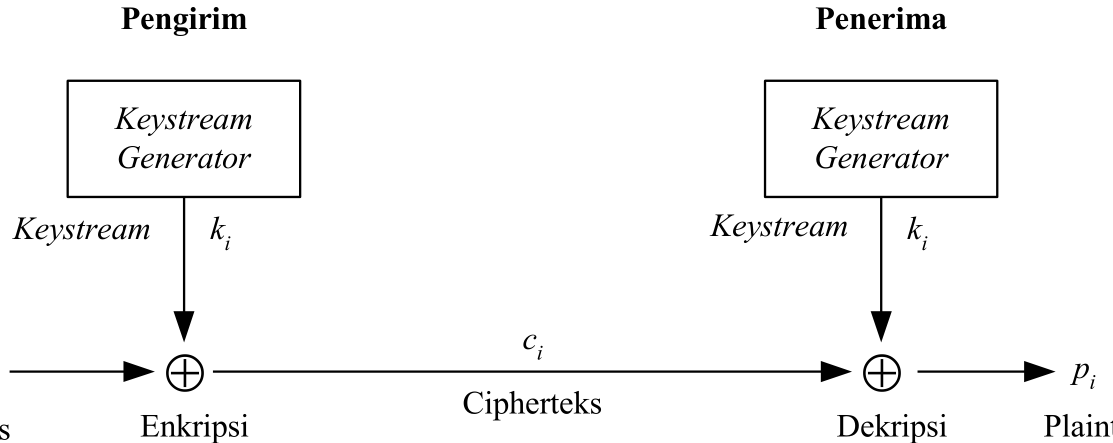
\includegraphics[width=121.80mm,height=121.77mm]{images/llm/page_026_img_01.png}%
\end{textblock*}

\newpage

% --- unit llm 27 ---
% === Halaman 27 (llm) ===

\section*{Keystream Generator}

\begin{itemize}
    \item \textit{Keystream generator} diimplementasikan sebagai prosedur yang sama baik di sisi pengirim maupun di sisi penerima pesan.
    \item \textit{Keystream generator} dapat membangkitkan \textit{keystream} dalam satuan bit, atau \textit{byte}, atau blok bit.
    \item Bit-bit \textit{keystream} adalah bit-bit acak, namun bukan \textit{true random}, tetapi \textit{pseudo-random}, karena bit-bit \textit{keystream} dapat dibangkitkan ulang baik di sisi pengirim maupun di sisi penerima pesan asalkan umpan (\textit{seed}) U yang digunakan sama.
    \item Bit-bit \textit{pseudo-random} memiliki periode (dapat terulang kembali setelah beberapa kali iterasi)
\end{itemize}

\newpage

% --- unit llm 28 ---
% === Halaman 28 (llm) ===

\begin{itemize}
    \item \textit{Keystream generator} menerima masukan sebuah umpan (\textit{seed}) $U$. Luaran dari prosedur merupakan fungsi dari $U$ (lihat Gambar 2). Pengirim dan penerima harus memiliki umpan $U$ yang sama. Umpan $U$ ini harus dijaga kerahasiaannya. Umpan $U$ dapat dianggap sebagai kunci eksternal.
    \item \textit{Keystream generator} menghasilkan bit-bit kunci yang di-XOR-kan dengan bit plainteks.
\end{itemize}

\vspace{40mm}

\textbf{Gambar 2} \textit{Cipher} aliran dengan pembangkit bit kunci-alir yang bergantung pada kunci $U$ [MEY82].

% deskripsi: Diagram blok sistem kriptografi stream cipher yang menunjukkan proses enkripsi oleh pengirim dan dekripsi oleh penerima menggunakan Keystream Generator dengan seed U.
% bbox normalisasi: [0.1800, 0.4100, 0.8600, 0.8500]
\begin{textblock*}{142.80mm}(37.80mm,121.77mm)
\noindent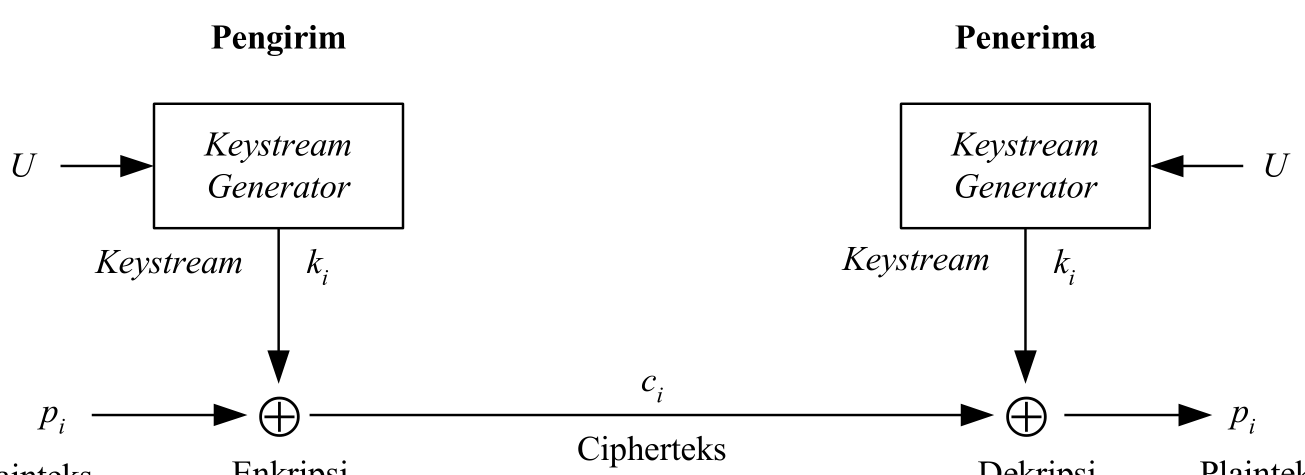
\includegraphics[width=142.80mm,height=130.68mm]{images/llm/page_028_img_01.png}%
\end{textblock*}

\newpage

% --- unit llm 29 ---
% === Halaman 29 (llm) ===

\begin{itemize}
  \item Contoh: Misalkan $U = 1111$
\end{itemize}

Algoritma sederhana memperoleh \textit{keystream} di dalam \textit{keystream generator} misalnya adalah sebagai berikut:

\textcolor{red}{XOR-kan bit ke-1 dengan bit ke-4 dari empat bit sebelumnya:}

\vspace{10mm}

\textcolor{blue}{111101011001000}111101011... \quad 111101...

\vspace{5mm}

dan akan berulang setiap 15 bit.

\begin{itemize}
  \item Secara umum, jika panjang $U$ adalah $n$ bit, maka bit-bit kunci tidak akan berulang sampai $2^n - 1$ bit.
\end{itemize}

\[ 111101011001000 \]

% deskripsi: Ilustrasi operasi XOR antara bit pertama dan keempat dari rangkaian bit untuk menghasilkan bit berikutnya dalam keystream generator.
% bbox normalisasi: [0.5600, 0.4500, 0.6400, 0.6100]
\begin{textblock*}{16.80mm}(117.60mm,133.65mm)
\noindent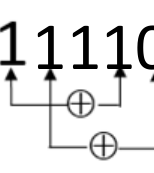
\includegraphics[width=16.80mm,height=47.52mm]{images/llm/page_029_img_01.png}%
\end{textblock*}

\newpage

% --- unit llm 30 ---
% === Halaman 30 (llm) ===

\begin{itemize}
    \item Misalkan plainteks adalah:
    \[ P: 0101\ 0111\ 0001\ 1001\ 0110\ 0100...\ (571964\text{ dalam Hexa}) \]
    Keystream yang dibangkitkan:
    \[ K: 111101011001001000111101011... \]
    \item Enkripsi: $C = P \oplus K$
    \vspace{10mm}
    \item Dekripsi: $P = C \oplus K$
    \vspace{10mm}
\end{itemize}

\vspace{49.60mm}

% deskripsi: Ilustrasi perhitungan operasi XOR antara plainteks P dan keystream K untuk mendapatkan cipherteks C, lengkap dengan konversi hasil biner ke hexadecimal.
% bbox normalisasi: [0.1770, 0.4150, 0.6500, 0.6300]
\begin{textblock*}{99.33mm}(37.17mm,123.25mm)
\noindent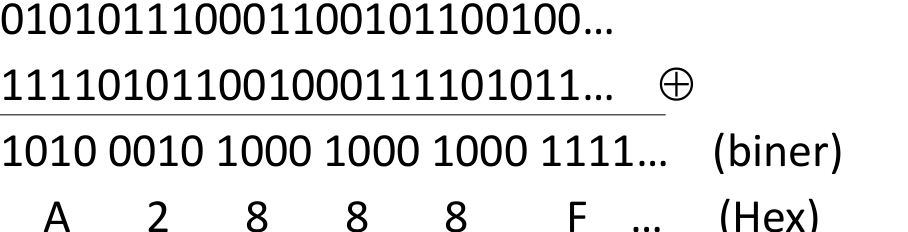
\includegraphics[width=99.33mm,height=63.86mm]{images/llm/page_030_img_01.png}%
\end{textblock*}

% deskripsi: Ilustrasi perhitungan operasi XOR antara cipherteks C dan keystream K untuk mengembalikan plainteks P awal dalam bentuk biner dan hexadecimal.
% bbox normalisasi: [0.1770, 0.7180, 0.7700, 0.8850]
\begin{textblock*}{124.53mm}(37.17mm,213.25mm)
\noindent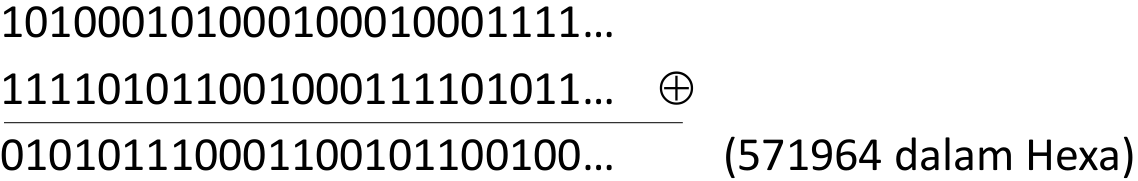
\includegraphics[width=124.53mm,height=49.60mm]{images/llm/page_030_img_02.png}%
\end{textblock*}

\newpage

% --- unit llm 31 ---
% === Halaman 31 (llm) ===

\begin{itemize}
  \item Karakteristik \textit{cipher}alir adalah melokalisir kesalahan enkripsi/dekripsi hanya pada bit yang eror saja.
  \item Maksudnya, kesalahan 1-bit pada cipherteks hanya menghasilkan kesalahan 1-bit pada plainteks hasil dekripsi.
  \item Misalkan cipherteks $1010\, \mathbf{0}010\, 1000\, 1000\, 1000\, 1111$ (Hex: A2888F) mengalami eror pada bit ke-5 dari semula 0 menjadi 1: $1010\, \mathbf{1}010\, 1000\, 1000\, 1000\, 1111$
  \item Ketika didekripsi:
\end{itemize}

\vspace{5mm}

\begin{align*}
\text{C: } & 1010\mathbf{1}0101000100010001111... \\
\text{K: } & 111101011001000111101011... \oplus \\
\hline
& 0101\mathbf{1}1110001100101100100... \quad (5\mathbf{F}1964\text{ dalam Hexa}) \\
& \quad \quad \quad \quad \quad \quad \quad \quad \text{(Seharusnya: 571964 dalam Hexa)}
\end{align*}

\newpage

% --- unit llm 32 ---
% === Halaman 32 (llm) ===

\section*{Feedback Shift Register (FSR)}

\begin{itemize}
    \item FSR adalah contoh sebuah \textit{keystream generator}.
    \item Umumnya diimplementasikan sebagai \textit{hardware}.
    \item FSR terdiri dari dua bagian: register geser (n bit) dan fungsi umpan balik
\end{itemize}

\vspace{50mm}

Fungsi umpan baik : $f(b_n, b_{n-1}, b_2, b_1)$
\[ b_n = f(b_n, b_{n-1}, b_2, b_1) \]

% deskripsi: Diagram blok Feedback Shift Register (FSR) yang menunjukkan register geser dengan bit b_n hingga b_1 dan kotak fungsi umpan-balik (feedback function) yang menerima input dari beberapa bit register dan memberikan output kembali ke bit b_n.
% bbox normalisasi: [0.1570, 0.4960, 0.7600, 0.7860]
\begin{textblock*}{126.63mm}(32.97mm,147.31mm)
\noindent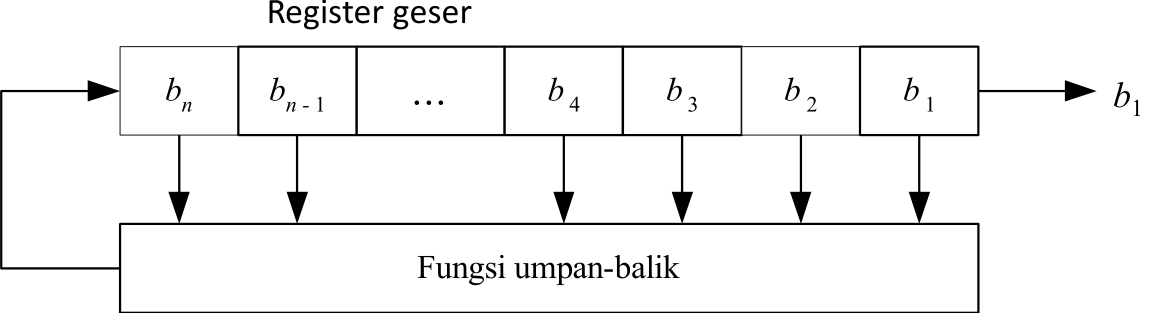
\includegraphics[width=126.63mm,height=86.13mm]{images/llm/page_032_img_01.png}%
\end{textblock*}

\newpage

% --- unit llm 33 ---
% === Halaman 33 (llm) ===

\begin{itemize}
    \item Contoh FSR adalah LFSR (\textit{Linear Feedback Shift Register})
\end{itemize}

\vspace{50mm}

\[ b_n = b_n \oplus b_{n-1} \oplus ... \oplus b_2 \oplus b_1 \]

\begin{itemize}
    \item Bit-bit di dalam register digeser satu bit ke kanan setiap kali pembangkitan bit luaran (= bit kunci alir atau \textit{keystream})
    \item Bit $b_n$ digeser ke tempat $b_{n-1}$, $b_{n-1}$ digeser ke $b_{n-2}$, dst, $b_2$ digeser ke $b_1$, $b_1$ terlempar ke luar
    \item Bit yang terlempar keluar ($b_1$) menjadi bit luaran LFSR
    \item Selanjutnya dihitung $b_n$ yang baru, yaitu $b_n = b_n \oplus b_{n-1} \oplus ... \oplus b_2 \oplus b_1$
\end{itemize}

% deskripsi: Diagram blok Register Geser (LFSR) yang menunjukkan pergeseran bit dari bn hingga b1 dengan jalur feedback menggunakan operasi XOR.
% bbox normalisasi: [0.1500, 0.1500, 0.7700, 0.4500]
\begin{textblock*}{130.20mm}(31.50mm,44.55mm)
\noindent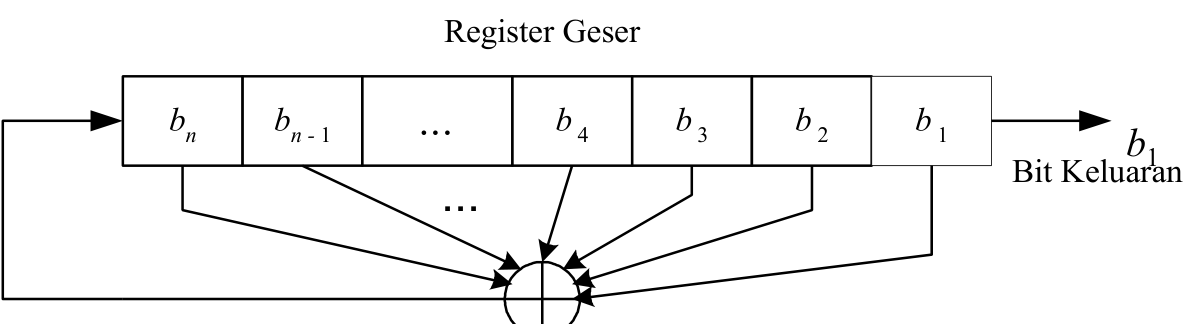
\includegraphics[width=130.20mm,height=89.10mm]{images/llm/page_033_img_01.png}%
\end{textblock*}

\newpage

% --- unit llm 34 ---
% === Halaman 34 (llm) ===

\begin{itemize}
  \item Contoh LFSR 4-bit
\end{itemize}

\vspace{40mm}

\begin{itemize}
  \item Fungsi umpan balik:
  \[ b_4 = f(b_1, b_4) = b_1 \oplus b_4 \]
\end{itemize}

% deskripsi: Diagram blok Linear Feedback Shift Register (LFSR) 4-bit yang menunjukkan pergeseran bit dari b4 ke b1 dan fungsi XOR sebagai umpan balik.
% bbox normalisasi: [0.2060, 0.2710, 0.6840, 0.5340]
\begin{textblock*}{100.38mm}(43.26mm,80.49mm)
\noindent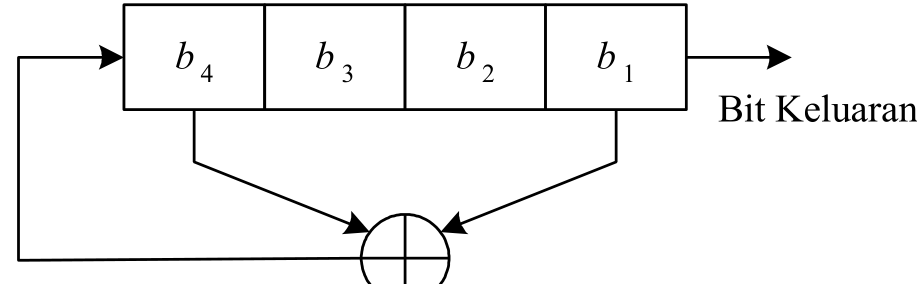
\includegraphics[width=100.38mm,height=78.11mm]{images/llm/page_034_img_01.png}%
\end{textblock*}

\newpage

% --- unit llm 35 ---
% === Halaman 35 (llm) ===

\vspace{193.05mm}

\begin{itemize}
    \item Contoh: jika LFSR 4-bit diinisialisasi dengan $U = 1111$
\end{itemize}

\vspace{10mm}

\begin{itemize}
    \item Barisan bit acak: $1\ 1\ 1\ 1\ 0\ 1\ 0\ 1\ 1\ 0\ 0\ 1\ 0\ 0\ 0\ \dots$
    \item Periode LFSR n-bit: $2^n - 1$
\end{itemize}

% deskripsi: Tabel yang menunjukkan proses perubahan isi register dan bit keluaran dari LFSR 4-bit selama 15 siklus (i=0 hingga i=15).
% bbox normalisasi: [0.2200, 0.1300, 0.6400, 0.7800]
\begin{textblock*}{88.20mm}(46.20mm,38.61mm)
\noindent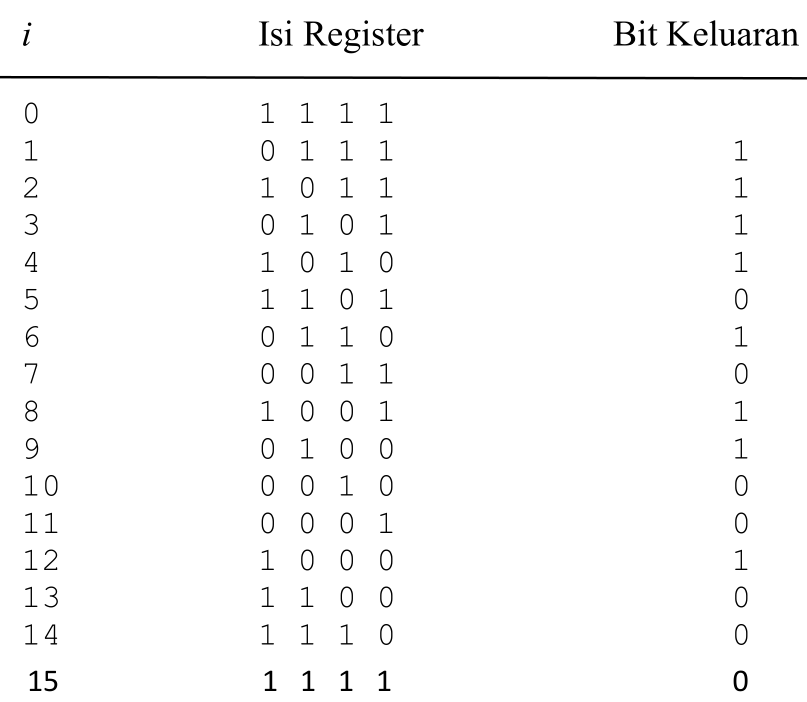
\includegraphics[width=88.20mm,height=193.05mm]{images/llm/page_035_img_01.png}%
\end{textblock*}

\newpage

% --- unit llm 36 ---
% === Halaman 36 (llm) ===

\section*{Aplikasi Cipher Alir}

\begin{itemize}
    \item \textit{Cipher} alir cocok untuk mengenkripsi aliran data yang kontinu melalui saluran komunikasi, misalnya:
    \begin{enumerate}
        \item Mengenkripsi data pada saluran yang menghubungkan antara dua buah komputer.
        \item Mengenkripsi suara pada jaringan telepon \textit{mobile} GSM.
    \end{enumerate}
    \item Alasan: jika bit cipherteks yang diterima mengandung kesalahan, maka hal ini hanya menghasilkan satu bit kesalahan pada waktu dekripsi, karena tiap bit plainteks ditentukan hanya oleh satu bit cipherteks.
    \item Selain itu, alasannya karena \textit{cipher} alir itu komputasinya cepat (dibutuhkan untuk \textit{real-time processing})
    \end{itemize}

\newpage

% --- unit llm 37 ---
% === Halaman 37 (llm) ===

\section*{Beberapa cipher alir dan tahun pembuatan}

\begin{itemize}
    \item RC4 (1987)
    \item A5 (1989)
    \item Rabbit (2003)
    \item Trivium (2004)
    \item SEAL (1997)
    \item Salsa20 (2004)
    \item Scream (2002)
    \item SOBER-128 (2003)
    \item WAKE (2003)
\end{itemize}

\begin{itemize}
    \item Turing (2000-2003)
    \item Scream (2002)
    \item VEST (2005)
    \item SNOW (2003)
    \item CryptMT (2005)
    \item FISH (1993)
    \item Grain (2004)
    \item Isaac (1995)
    \item MICKEY (2004)
\end{itemize}

\newpage

% --- unit llm 38 ---
% === Halaman 38 (llm) ===

% (tidak ada teks dari model)

% deskripsi: Tabel perbandingan berbagai stream cipher yang mencakup kolom Stream cipher, Creation date, Speed, Effective key-length, Initialization vector, Internal state, Best known attack, dan Computational complexity.
% bbox normalisasi: [0.0800, 0.3300, 0.9300, 0.9600]
\begin{textblock*}{178.50mm}(16.80mm,98.01mm)
\noindent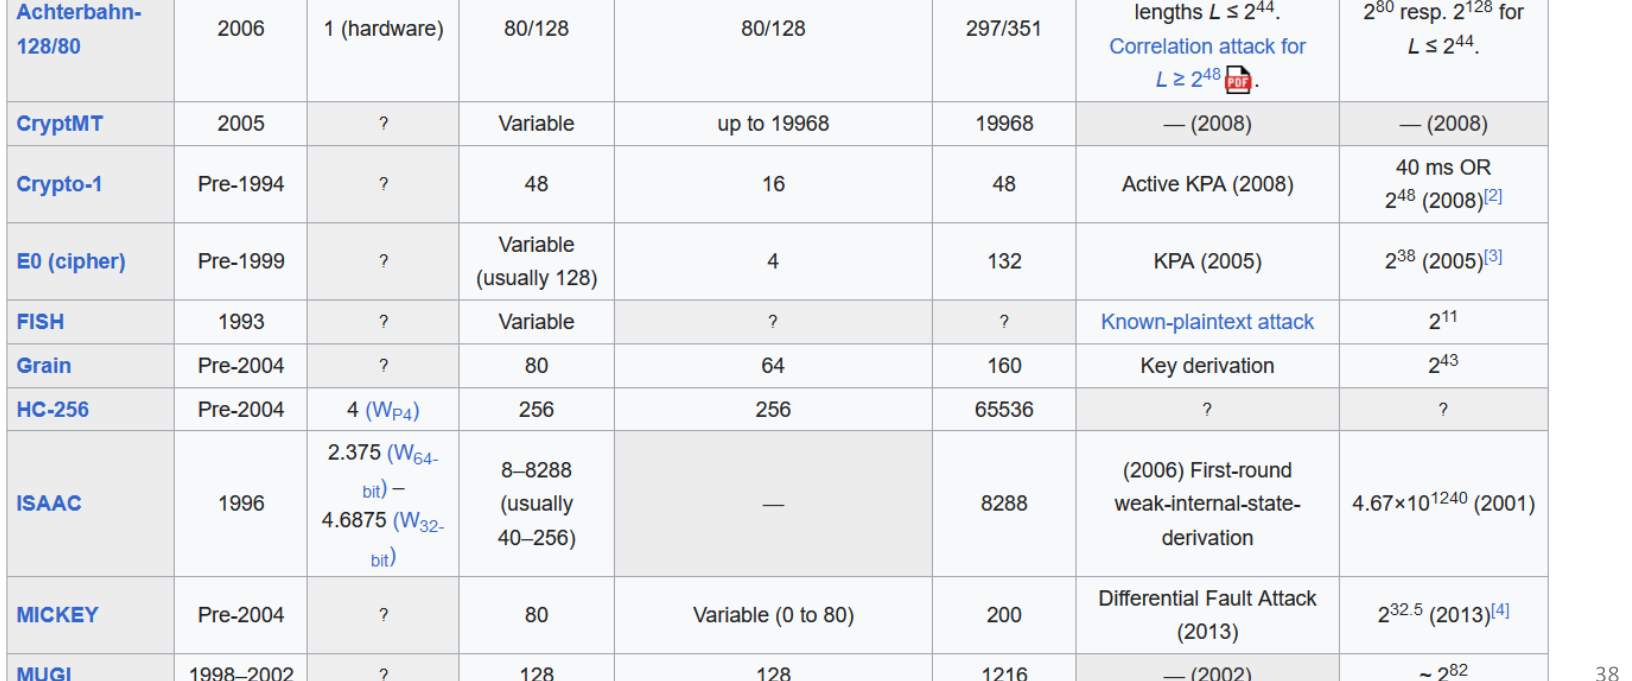
\includegraphics[width=178.50mm,height=187.11mm]{images/llm/page_038_img_01.png}%
\end{textblock*}

\newpage

% --- unit llm 39 ---
% === Halaman 39 (llm) ===

\vspace{276.21mm}

(Sumber: https://en.wikipedia.org/wiki/Stream_cipher)

% deskripsi: Tabel perbandingan berbagai stream cipher yang mencakup kolom nama cipher, tahun rilis, panjang kunci, panjang nonce/IV, panjang state, periode, serangan/kelemahan, dan kompleksitas serangan.
% bbox normalisasi: [0.0000, 0.0000, 0.8350, 0.9300]
\begin{textblock*}{175.35mm}(0.00mm,0.00mm)
\noindent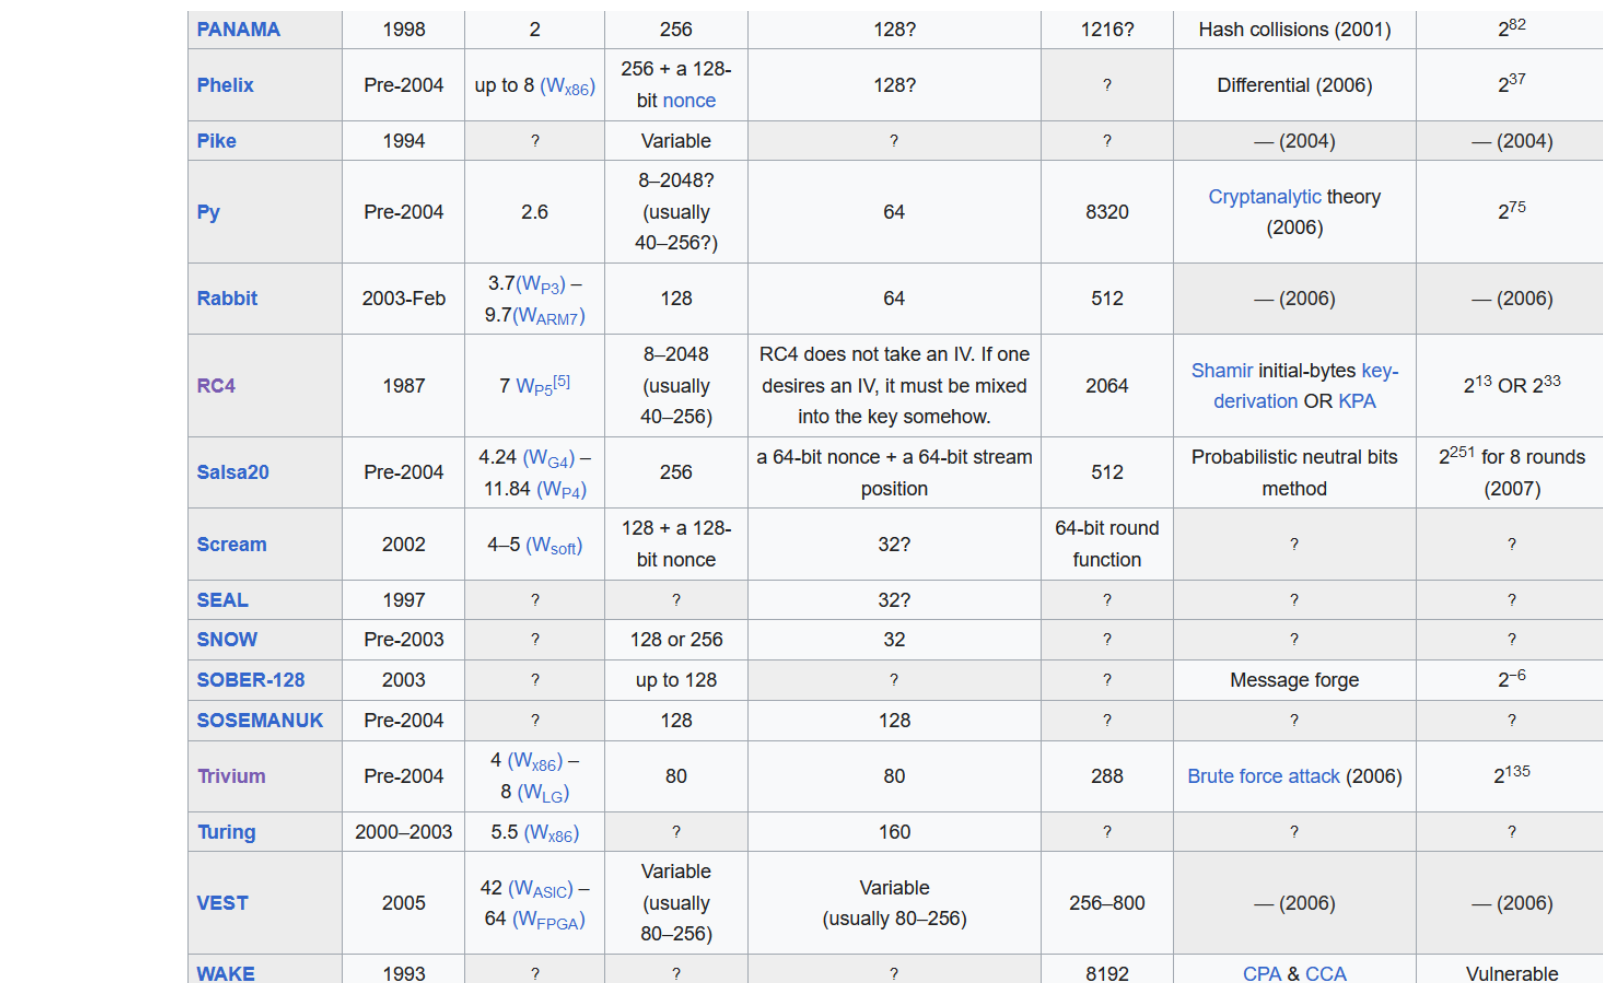
\includegraphics[width=175.35mm,height=276.21mm]{images/llm/page_039_img_01.png}%
\end{textblock*}

\newpage

% --- unit llm 40 ---
% === Halaman 40 (llm) ===

\section*{1. RC4}

\begin{itemize}
    \item \textit{Cipher}alir yang paling popular, namun sekarang sudah tidak aman
    \item Dibuat oleh Ronald Rivest (1987) dari Laboratorium RSA
    \item \textit{RC} adalah singkatan dari \textit{Ron's Code}. Versi lain mengatakan \textit{Rivest Cipher}.
    \item Digunakan di dalam beberapa sistem keamanan seperti:
    \begin{itemize}
        \item protokol SSL (\textit{Secure Socket Layer}) dan TLS (\textit{Transport Layer Security})
        \item Standard IEEE 802.11 \textit{wireless} LAN: WEP (\textit{Wired Equivalent Privacy})
        \item WPA (\textit{Wi-fi Protocol Access}) untuk nirkabel
    \end{itemize}
\end{itemize}

\newpage

% --- unit llm 41 ---
% === Halaman 41 (llm) ===

\section*{Ron Rivest}

"Rivest" redirects here. For other people with the same name, see Rivest (surname).

\vspace{193.05mm}

\textbf{Ronald Linn Rivest} (/r\textsuperscript{\textregistered}vest/)$^{[3][4]}$ born May 6, 1947) is an American cryptographer and computer scientist whose work has spanned the fields of algorithms and combinatorics, cryptography, machine learning, and election integrity. He is an Institute Professor at the Massachusetts Institute of Technology (MIT)$^{[5]}$ and a member of MIT's Department of Electrical Engineering and Computer Science and its Computer Science and Artificial Intelligence Laboratory.

\vspace{50mm}

Along with Adi Shamir and Len Adleman, Rivest is one of the inventors of the RSA algorithm, for which they won the 2002 ACM Turing Award. He is also the inventor of the symmetric key encryption algorithms RC2, RC4, and RC5, and co-inventor of RC6. He also devised the MD2, MD4, MD5 and MD6 cryptographic hash functions.

\subsection*{Education [ edit ]}

Rivest earned a bachelor's degree in mathematics from Yale

% deskripsi: Infobox Wikipedia tentang Ron Rivest yang berisi foto, tanggal lahir, lokasi kelahiran, pendidikan, dan pencapaian utama.
% bbox normalisasi: [0.5560, 0.2860, 0.8040, 0.9360]
\begin{textblock*}{52.08mm}(116.76mm,84.94mm)
\noindent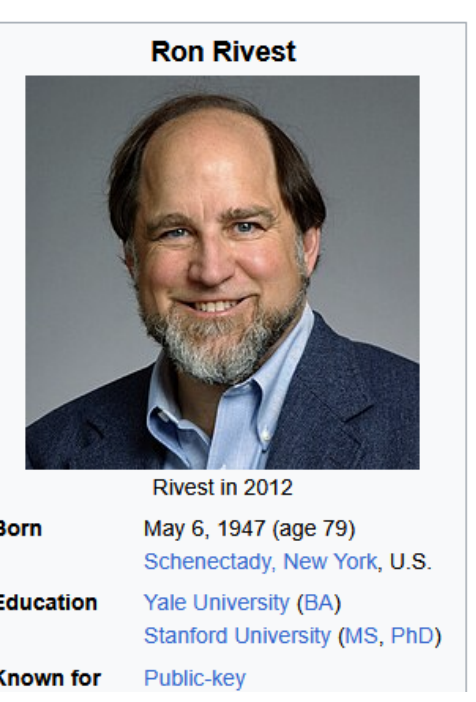
\includegraphics[width=52.08mm,height=193.05mm]{images/llm/page_041_img_01.png}%
\end{textblock*}

\newpage

% --- unit llm 42 ---
% === Halaman 42 (llm) ===

\vspace{139.59mm}

Diagram Blok RC4:\vspace{60mm}
\begin{itemize}
    \item Kunci rahasia (\textit{secret key}) memiliki panjang maksimal 256 karakter (1 karakter = 1byte). Jika panjang kunci kurang dari 256 \textit{byte} maka karakter-karakter kunci diulang secara periodik.
    \item RC4 menghasilkan luaran berupa kunci-alir (\textit{keystream}) dengan panjang tak terbatas
\end{itemize}

% deskripsi: Diagram blok proses enkripsi RC4 yang menunjukkan aliran dari Secret Key melalui blok RC4 untuk menghasilkan Keystream, yang kemudian di-XOR (simbol plus dalam lingkaran) dengan Plaintext untuk menghasilkan Ciphertext.
% bbox normalisasi: [0.1000, 0.1900, 0.7500, 0.6600]
\begin{textblock*}{136.50mm}(21.00mm,56.43mm)
\noindent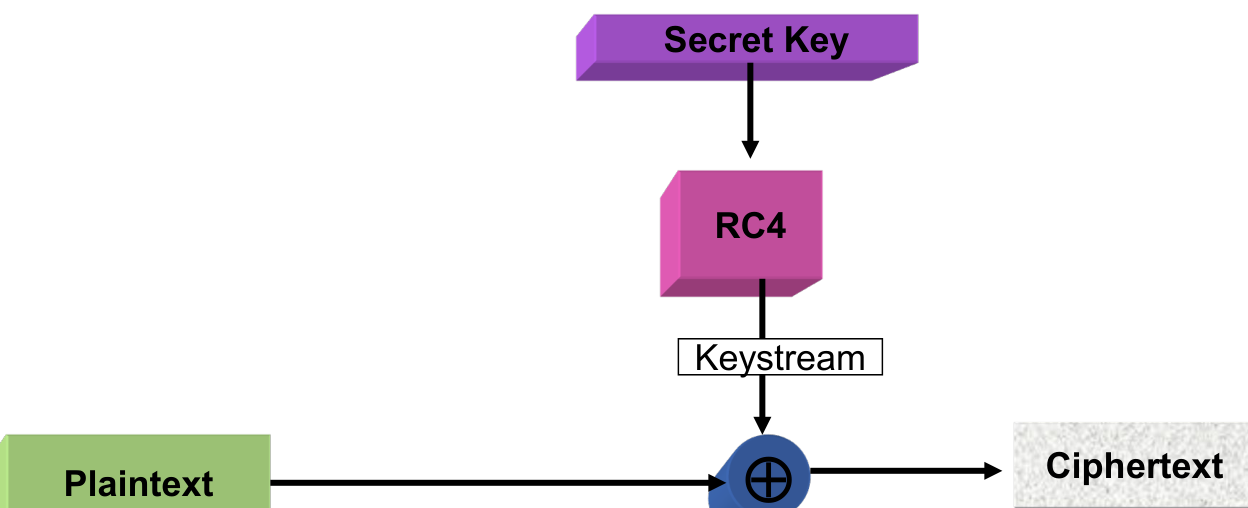
\includegraphics[width=136.50mm,height=139.59mm]{images/llm/page_042_img_01.png}%
\end{textblock*}

\newpage

% --- unit llm 43 ---
% === Halaman 43 (llm) ===

\begin{itemize}
    \item RC4 membangkitkan kunci-alir (\textit{keystream}) dalam satuan \textit{byte} setiap kalinya, yang kemudian di-XOR-kan dengan \textit{byte} plainteks (operasi \textit{bitwise XOR})
    \item Untuk membangkitkan kunci-alir, \textit{cipher} menggunakan status internal yang terdiri dari:
    \begin{itemize}
        \item Larik $S_0, S_1, ..., S_{255}$. Elemen-elemen di dalam larik S dipermutasi berdasarkan kunci rahasia $K$ dengan panjang variabel.
        \item Dua buah pencacah indeks, $i$ dan $j$
    \end{itemize}
    \item RC4 terdiri dari dua sub-proses:
    \begin{enumerate}
        \item \textit{Key-Scheduling Algorithm} (KSA)
        \item \textit{Pseudo-random generation algorithm} (PRGA).
    \end{enumerate}
\end{itemize}

\newpage

% --- unit llm 44 ---
% === Halaman 44 (llm) ===

\section*{Key-Scheduling Algorithm (KSA)}

\begin{enumerate}
    \item Inisialisasi larik $\text{S}: \text{S}_0 = 0, \text{S}_1 = 1, ..., \text{S}_{255} = 255$

    \vspace{10mm}

    \begin{verbatim}
    for i <- 0 to 255 do
        S[i] <- i
    end
    \end{verbatim}
\end{enumerate}

% deskripsi: Representasi visual array S yang diinisialisasi dengan nilai urut dari 0 sampai 255
% bbox normalisasi: [0.1200, 0.7000, 0.7680, 0.8050]
\begin{textblock*}{136.08mm}(25.20mm,207.90mm)
\noindent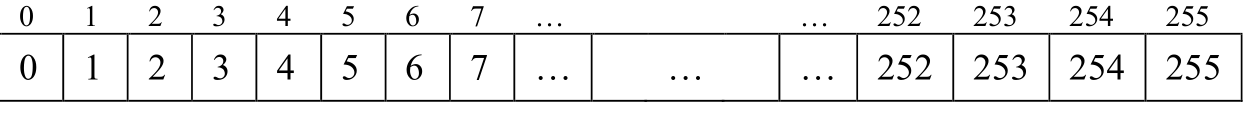
\includegraphics[width=136.08mm,height=31.19mm]{images/llm/page_044_img_01.png}%
\end{textblock*}

\newpage

% --- unit llm 45 ---
% === Halaman 45 (llm) ===

3. Lakukan pengacakan (permutasi) nilai-nilai di dalam larik S berdasarkan kunci rahasia K (kunci eksternal dari pengguna):

\vspace{5mm}

\begin{itemize}
    \item Permutasi ini menyebabkan elemen-elemen di dalam larik S teracak.
    \item $\text{K[i mod Length(K)]}$ menyatakan karakter-karakter kunci diulang secara periodik jika panjangnya kurang dari 256
\end{itemize}

% deskripsi: Potongan kode pseudocode untuk melakukan permutasi pada larik S menggunakan kunci K.
% bbox normalisasi: [0.1480, 0.2940, 0.8670, 0.5810]
\begin{textblock*}{150.99mm}(31.08mm,87.32mm)
\noindent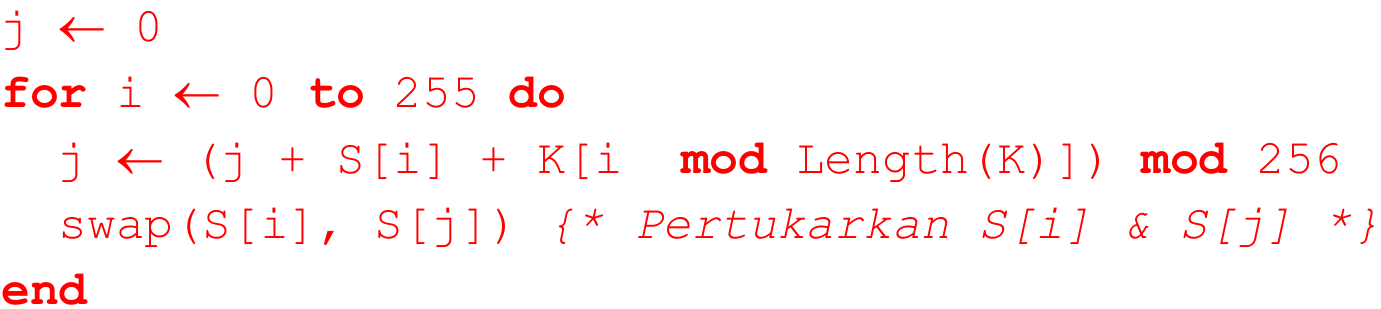
\includegraphics[width=150.99mm,height=85.24mm]{images/llm/page_045_img_01.png}%
\end{textblock*}

\newpage

% --- unit llm 46 ---
% === Halaman 46 (llm) ===

\section*{Pseudo-random generation algorithm (PRGA)}

\vspace{64.15mm}

\begin{itemize}
    \item PRGA membangkitkan kunci-alir (\textit{keystream}) dengan cara mengambil nilai $S[i]$ dan $S[j]$, mempertukarkannya, lalu menjumlahkan keduanya dalam modulus 256.
    \item Kunci alir tersebut kemudian di-XOR-kan dengan sebuah karakter plainteks.
\end{itemize}

\vspace{10mm}

\begin{verbatim}
i <- 0
j <- 0
for idx <- 0 to Length(P) - 1 do
    i <- (i + 1) mod 256
    j <- (j + S[i]) mod 256
    swap(S[i], S[j])    {* Pertukarkan nilai S[i] dan S[j] *}
    t <- (S[i] + S[j]) mod 256
    u <- S[t]           (* keystream *)
    c <- u XOR P[idx]   { enkripsi }
end
\end{verbatim}

% deskripsi: Diagram ilustrasi proses PRGA yang menunjukkan array S dengan indeks i, j, dan t, serta operasi swap dan penjumlahan modulo 256.
% bbox normalisasi: [0.5110, 0.3690, 0.9780, 0.5850]
\begin{textblock*}{98.07mm}(107.31mm,109.59mm)
\noindent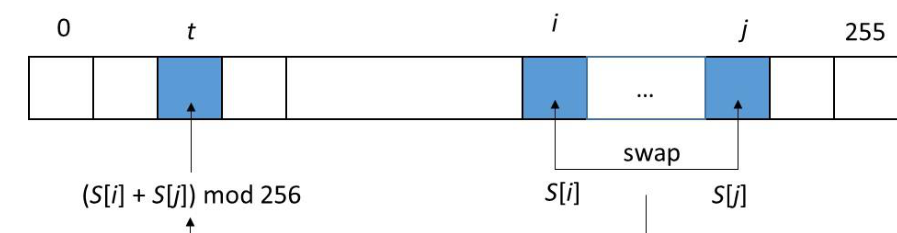
\includegraphics[width=98.07mm,height=64.15mm]{images/llm/page_046_img_01.png}%
\end{textblock*}

\newpage

% --- unit llm 47 ---
% === Halaman 47 (llm) ===

% (tidak ada teks dari model)

% deskripsi: Diagram ilustrasi algoritma RC4 yang menunjukkan proses pemutakhiran S-box, termasuk operasi swap antara elemen S[i] dan S[j], serta penghitungan indeks t menggunakan rumus (S[i] + S[j]) mod 256.
% bbox normalisasi: [0.1500, 0.2500, 0.8500, 0.6000]
\begin{textblock*}{147.00mm}(31.50mm,74.25mm)
\noindent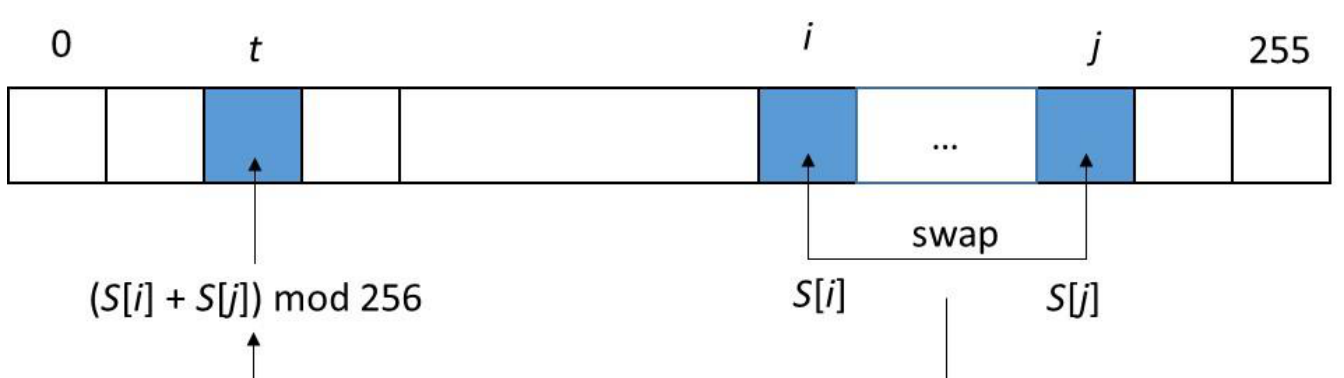
\includegraphics[width=147.00mm,height=103.95mm]{images/llm/page_047_img_01.png}%
\end{textblock*}

\newpage

% --- unit llm 48 ---
% === Halaman 48 (llm) ===

\vspace{92.07mm}

\section*{Operasi RC4 secara keseluruhan:}

\vspace{130.68mm}

% deskripsi: Diagram proses inisialisasi state dan kunci RC4, mencakup tahap 'State and key initialization' dan 'Initial state permutation'.
% bbox normalisasi: [0.2100, 0.1700, 0.6600, 0.4800]
\begin{textblock*}{94.50mm}(44.10mm,50.49mm)
\noindent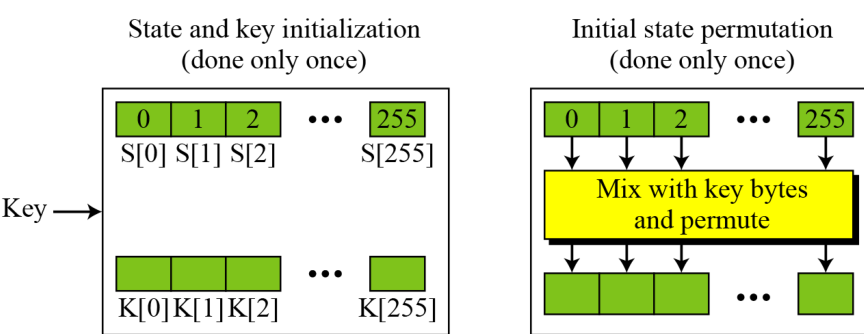
\includegraphics[width=94.50mm,height=92.07mm]{images/llm/page_048_img_01.png}%
\end{textblock*}

% deskripsi: Diagram proses pembuatan key stream RC4 melalui 'State permutation for key stream generation' dan operasi enkripsi XOR antara plaintext (P) dan key stream (k) untuk menghasilkan ciphertext (C).
% bbox normalisasi: [0.1100, 0.5400, 0.7300, 0.9800]
\begin{textblock*}{130.20mm}(23.10mm,160.38mm)
\noindent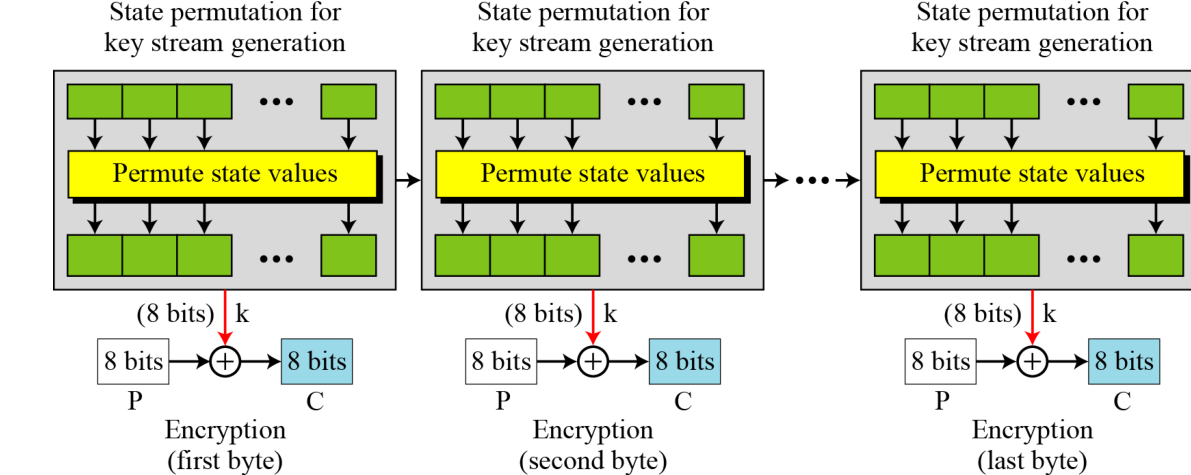
\includegraphics[width=130.20mm,height=130.68mm]{images/llm/page_048_img_02.png}%
\end{textblock*}

\newpage

% --- unit llm 49 ---
% === Halaman 49 (llm) ===

\section*{Keamanan RC4}

\begin{itemize}
    \item RC4 memiliki kelemahan, yaitu \textit{byte-byte} pada \textit{keystream} awal pembangkitan memiliki korelasi yang tinggi dengan beberapa \textit{byte} awal kunci
    \item Oleh karena itu direkomendasikan membuang 256 sampai 512 \textit{byte keystream} awal
    \item RC4 adalah \textit{cipher} alir, maka ia tidak kuat terhadap serangan seperti \textit{flip-bit attack} maupun serangan-serangan \textit{stream attack} lainnya.
    \item Saat ini keamanan RC4 sudah berhasil dipecahkan dalam hitungan jam atau hari.
    \item Pada bulan Februari 2015, RC4 dilarang penggunaannya di dalam \textit{Transport Layer Security} (TLS) seperti disebutkan di dalam RFC 7465 (\url{https://tools.ietf.org/html/rfc7465}).
    \item Beberapa varian RC4 telah dibuat untuk mengatasi kelemahannya, yaitu Spritz, RC4A, VMPC, dan RC4+.
\end{itemize}

\newpage

% --- unit llm 50 ---
% === Halaman 50 (llm) ===

\section*{Kode Program RC4 (dalam Bahasa C++)}

\vspace{172.26mm}

\begin{itemize}
    \item Enkripsi
\end{itemize}

\vspace{10mm}

% deskripsi: Screenshot cuplikan kode program C++ untuk implementasi enkripsi RC4 yang terbagi dalam dua kolom.
% bbox normalisasi: [0.0500, 0.3300, 0.9450, 0.9100]
\begin{textblock*}{187.95mm}(10.50mm,98.01mm)
\noindent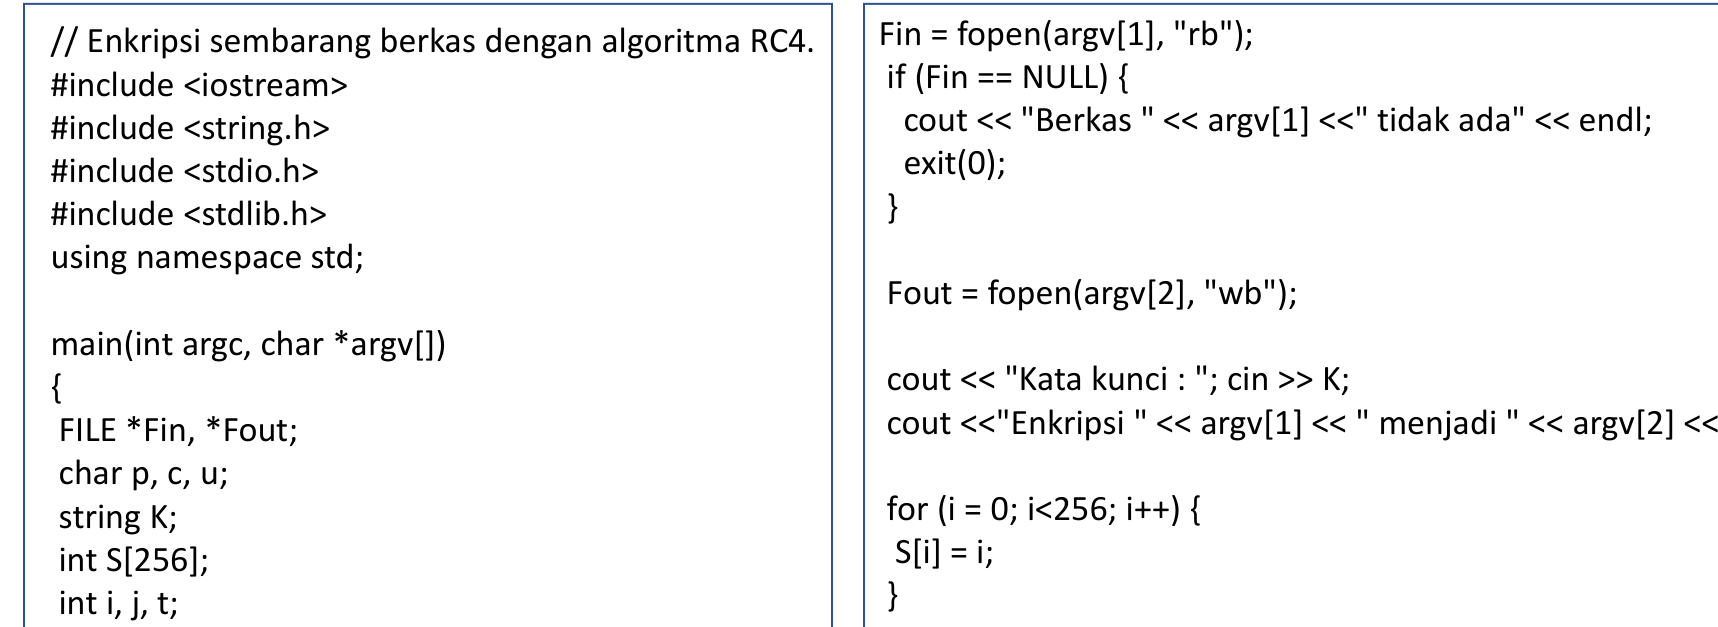
\includegraphics[width=187.95mm,height=172.26mm]{images/llm/page_050_img_01.png}%
\end{textblock*}

\newpage

% --- unit llm 51 ---
% === Halaman 51 (llm) ===

\begin{verbatim}
j = 0;
for (i=0; i<256; i++) {
  j = (j + S[i] + K[i % K.length()]) % 256;
  swap(S[i], S[j]); // Pertukarkan nilai S[i] dan S[j]
}

\vspace{170.48mm}

i = 0; j = 0;
while (!feof(Fin)) {
  p = fgetc(Fin);
  i = (i + 1) % 256;
  j = (j + S[i]) % 256;
  swap(S[i], S[j]); // Pertukarkan nilai S[i] dan S[j]
  t = (S[i] + S[j]) % 256;
  u = S[t]; // keystream
  c = u ^ p;
  fputc(c, Fout);
}
fclose(Fin); fclose(Fout);
\end{verbatim}

% deskripsi: Screenshot potongan kode program dalam bahasa C/C++ yang mengimplementasikan algoritma RC4 (KSA dan PRGA).
% bbox normalisasi: [0.1950, 0.2600, 0.6780, 0.8340]
\begin{textblock*}{101.43mm}(40.95mm,77.22mm)
\noindent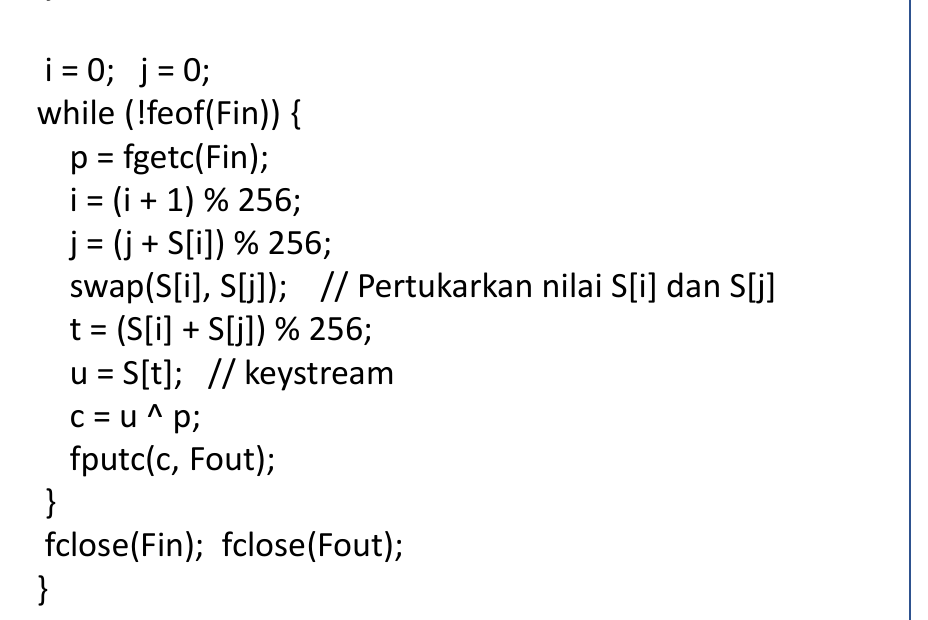
\includegraphics[width=101.43mm,height=170.48mm]{images/llm/page_051_img_01.png}%
\end{textblock*}

\newpage

% --- unit llm 52 ---
% === Halaman 52 (llm) ===

\section*{Dekripsi}

\vspace{10mm}

\begin{minipage}[t]{0.45\textwidth}
\begin{verbatim}
//Dekripsi sembarang berkas dengan algoritma RC4
#include <iostream>
#include <string.h>
#include <stdlib.h>
#include <stdio.h>
using namespace std;

main(int argc, char *argv[])
{
 FILE *Fin, *Fout;
 char p, c, u;
 string K;
 int S[256];
 int i, j, t;
\end{verbatim}
\end{minipage}
\hfill
\begin{minipage}[t]{0.45\textwidth}
\begin{verbatim}
Fin = fopen(argv[1], "rb");
if (Fin == NULL) {
 cout << "Berkas " << argv[1] <<" tidak ada" << endl;
 exit(0);
}

Fout = fopen(argv[2], "wb");

cout << "Kata kunci : "; cin >> K;
cout <<"Dekripsi " << argv[1] << " menjadi " << argv[2] << "...";

for (i = 0; i<256; i++){
 S[i] = i;
}
\end{verbatim}
\end{minipage}

% deskripsi: Screenshot potongan kode program C++ untuk proses dekripsi menggunakan algoritma RC4 yang terbagi dalam dua kolom.
% bbox normalisasi: [0.0400, 0.1800, 0.9800, 0.7800]
\begin{textblock*}{197.40mm}(8.40mm,53.46mm)
\noindent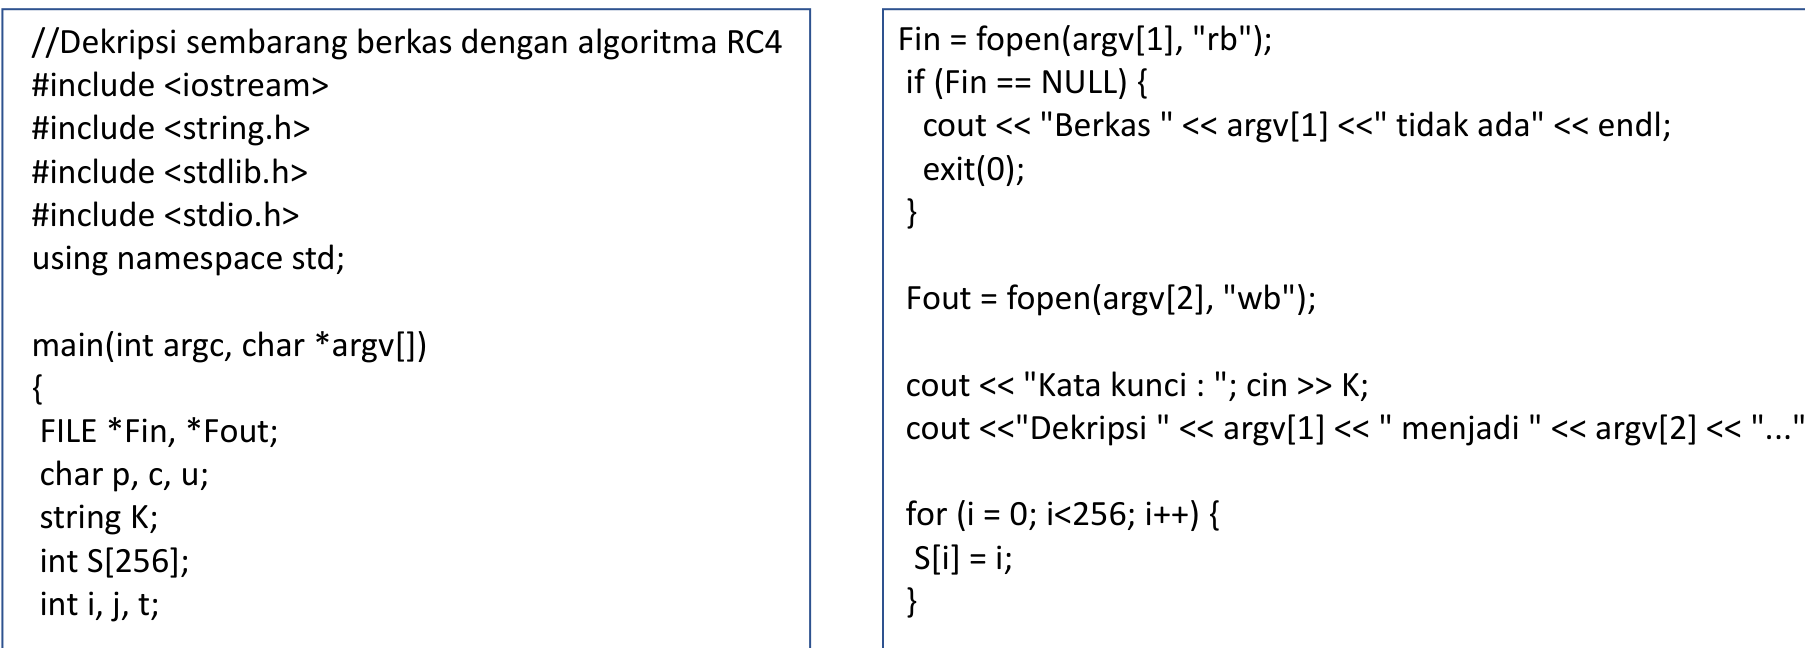
\includegraphics[width=197.40mm,height=178.20mm]{images/llm/page_052_img_01.png}%
\end{textblock*}

\newpage

% --- unit llm 53 ---
% === Halaman 53 (llm) ===

\vspace{119.99mm}

j = 0;\nfor (i=0; i<256; i++) {\n\t j = (j + S[i] + K[i \% K.length()]) \% 256;\n\t swap(S[i], S[j]); // Pertukarkan nilai S[i] dan S[j]\n}\n\ni = 0; j = 0;\nwhile (!leof(Fin)) {\n\t c = fgetc(Fin);\n\t i = (i + 1) \% 256;\n\t j = (j + S[i]) \% 256;\n\t swap(S[i], S[j]); // Pertukarkan nilai S[i] dan S[j]\n\t t = (S[i] + S[j]) \% 256;\n\t u = S[t]; // keystream\n\t p = u \^ c;\n\t fputc(p, Fout);\n}\nfclose(Fin); fclose(Fout);

% deskripsi: Potongan kode program implementasi algoritma RC4 dalam bahasa pemrograman C/C++.
% bbox normalisasi: [0.2140, 0.4600, 0.7670, 0.8640]
\begin{textblock*}{116.13mm}(44.94mm,136.62mm)
\noindent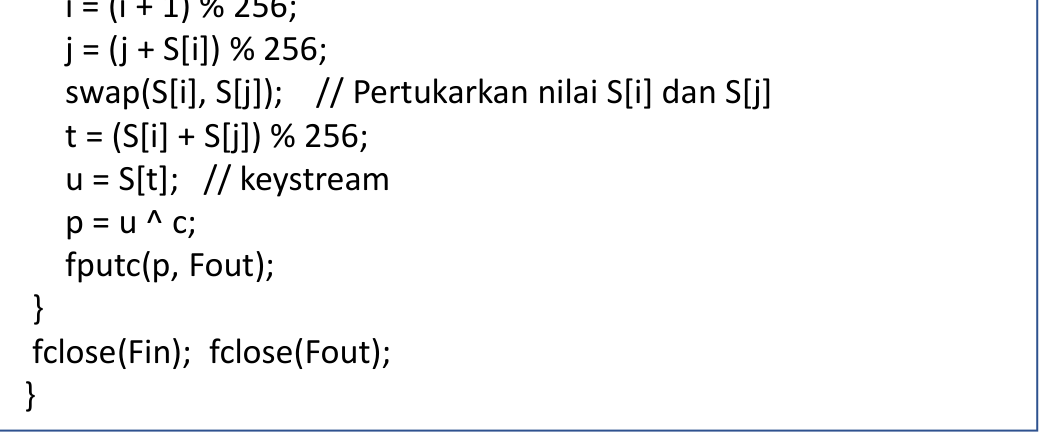
\includegraphics[width=116.13mm,height=119.99mm]{images/llm/page_053_img_01.png}%
\end{textblock*}

\newpage

% --- unit llm 54 ---
% === Halaman 54 (llm) ===

\section*{Demo RC4 Online}

\begin{enumerate}
  \item \url{https://crypt-online.ru/en/crypts/rc4/}
  \item \url{https://www.lddgo.net/en/encrypt/rc4}
\end{enumerate}

\newpage

% --- unit llm 55 ---
% === Halaman 55 (llm) ===

Enkripsi

\vspace{10mm}

\textbf{Crypt-Online}

Main $\Rightarrow$ Conversions $\Rightarrow$ RC4

\textbf{Encryptions}
\begin{itemize}
    \item Without a key
    \item Symmetric
    \begin{itemize}
        \item AES (Rijndael)
        \item DES
        \item RC4
    \end{itemize}
    \item Asymmetric
    \item Mathematical
    \item Utilities
\end{itemize}

% deskripsi: Screenshot antarmuka web encryptor RC4 yang menunjukkan input teks 'Terbanglah sampai ke angkasa setinggi bintang di langit', kunci 'Selamat sore gaess', dan hasil cipher text.
% bbox normalisasi: [0.2800, 0.3600, 0.7300, 0.9400]
\begin{textblock*}{94.50mm}(58.80mm,106.92mm)
\noindent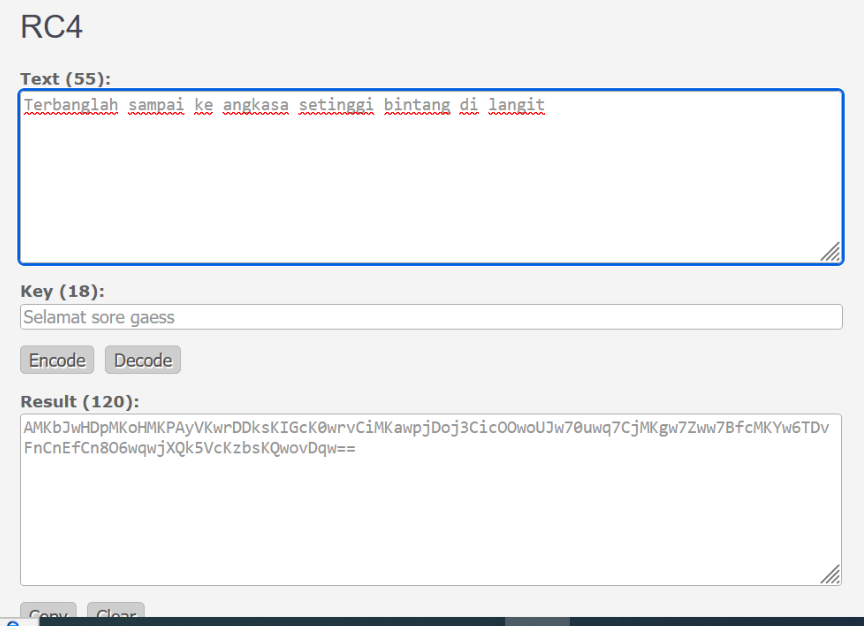
\includegraphics[width=94.50mm,height=172.26mm]{images/llm/page_055_img_01.png}%
\end{textblock*}

\newpage

% --- unit llm 56 ---
% === Halaman 56 (llm) ===

Dekripsi

\vspace{10mm}

\textbf{Crypt-Online}

Main | Conversions | Contacts

Main $\gg$ Conversions $\gg$ RC4

\textbf{Encryptions}
\begin{itemize}
    \item Without a key
    \item Symmetric
    \begin{itemize}
        \item AES (Rijndael)
        \item DES
        \item RC4
    \end{itemize}
    \item Asymmetric
    \item Mathematical
    \item Utilities
\end{itemize}

\textbf{RC4}

Text (120): \\
AMKBj4dpRmhCOKMHPaYVkwRrdDKsIGK0cWrvC1MKawpDoj3C1C00oWoUj70uwq7CJMKgW7zWw78FcMKyW6TDV\\
FnCnEFcN806wqwjxQXsKVcKzbsXKQwovDqw=

Key (18): \\
Selamat sore gaess

Encode | Decode

Result (55): \\
Terbanglah sampai ke angkasa setinggi bintang di langit

% deskripsi: Screenshot antarmuka situs web Crypt-Online yang menunjukkan proses dekripsi teks menggunakan algoritma RC4
% bbox normalisasi: [0.0680, 0.1400, 0.9600, 0.8600]
\begin{textblock*}{187.32mm}(14.28mm,41.58mm)
\noindent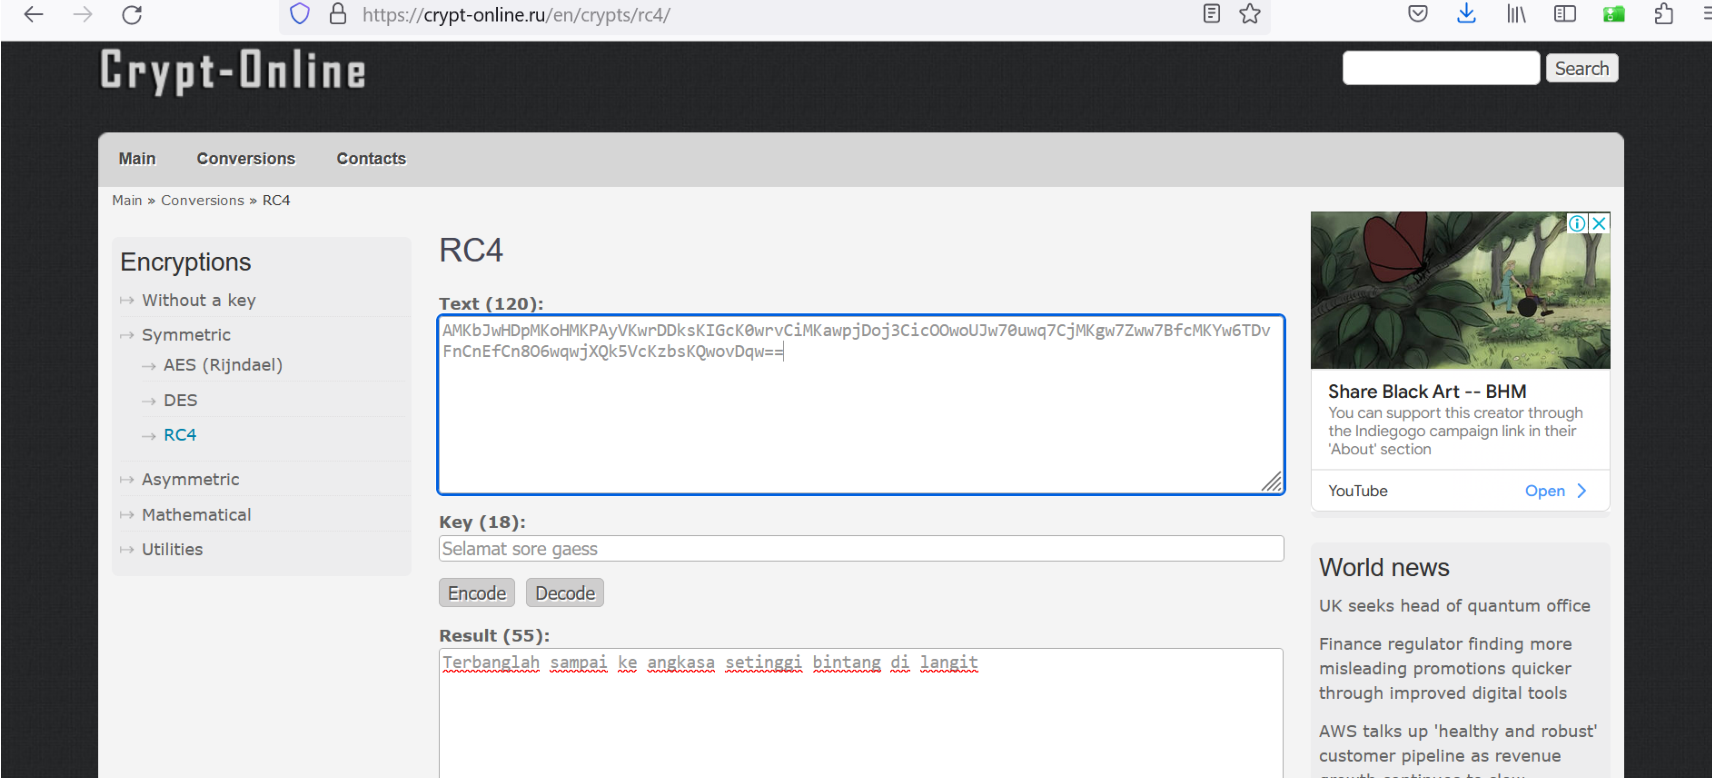
\includegraphics[width=187.32mm,height=213.84mm]{images/llm/page_056_img_01.png}%
\end{textblock*}

\newpage

% --- unit llm 57 ---
% === Halaman 57 (llm) ===

If you need to know about RC4 encryption algorithm, please carefully read the instructions of this tool to set relevant parameters correctly.

\vspace{207.90mm}

Input Content

Terbanglah sampai ke angkasa setinggi bintang di langit

\begin{tabular}{|l|l|l|l|}
\hline
Password & selamat sore gaes & Charset & UTF-8 \\ \hline
In-Format & string & Out-Format & hex \\ \hline
\end{tabular}

RC4 Encrypt RC4 Decrypt Copy Clear

Output Result

5cc0adeadf45a1c2a0cb1b6527f95afa1a1cfb73d5dbd7173933f49139a227b088f5d06f0e35fd3efd2cb220bb4e971b1cbeae4fa2f694dc

% deskripsi: Screenshot antarmuka web alat enkripsi dan dekripsi RC4 yang menunjukkan input teks, password, pengaturan format, dan hasil output hex.
% bbox normalisasi: [0.0300, 0.2000, 0.9400, 0.9000]
\begin{textblock*}{191.10mm}(6.30mm,59.40mm)
\noindent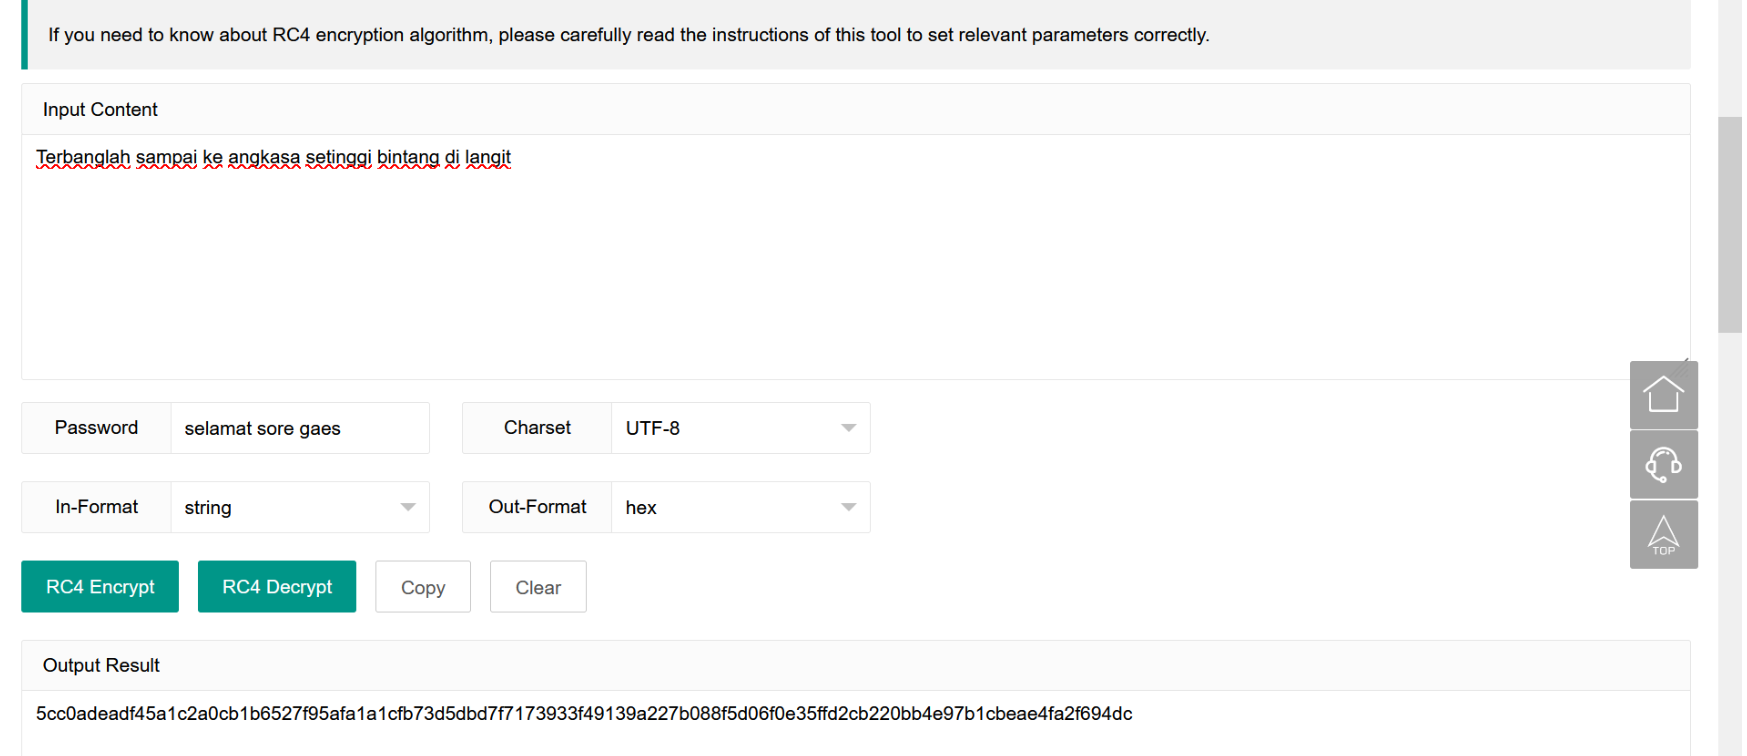
\includegraphics[width=191.10mm,height=207.90mm]{images/llm/page_057_img_01.png}%
\end{textblock*}

\newpage

% --- unit llm 58 ---
% === Halaman 58 (llm) ===

Dekripsi

\vspace{10mm}

If you need to know about RC4 encryption algorithm, please carefully read the instructions of this tool to set relevant parameters correctly.

Input Content

5cc0adeadf45a1c2a0cb1b6527f95afa1a1cfb73d5dbd7f7173933f49139a227b088f5d06f0e35fd2cb220bb44e97b1cbeae4fa2f694dc

Password: selamat sore gaes

Charset: UTF-8

In-Format: hex

Out-Format: string

RC4 Encrypt \quad RC4 Decrypt \quad Copy \quad Clear

Output Result

Terbanglah sampai ke angkasa setinggi bintang di langit

% deskripsi: Screenshot antarmuka web alat enkripsi dan dekripsi RC4 yang menunjukkan input ciphertext hex, password 'selamat sore gaes', dan hasil dekripsi teks 'Terbanglah sampai ke angkasa setinggi bintang di langit'.
% bbox normalisasi: [0.0600, 0.1000, 0.9500, 0.9100]
\begin{textblock*}{186.90mm}(12.60mm,29.70mm)
\noindent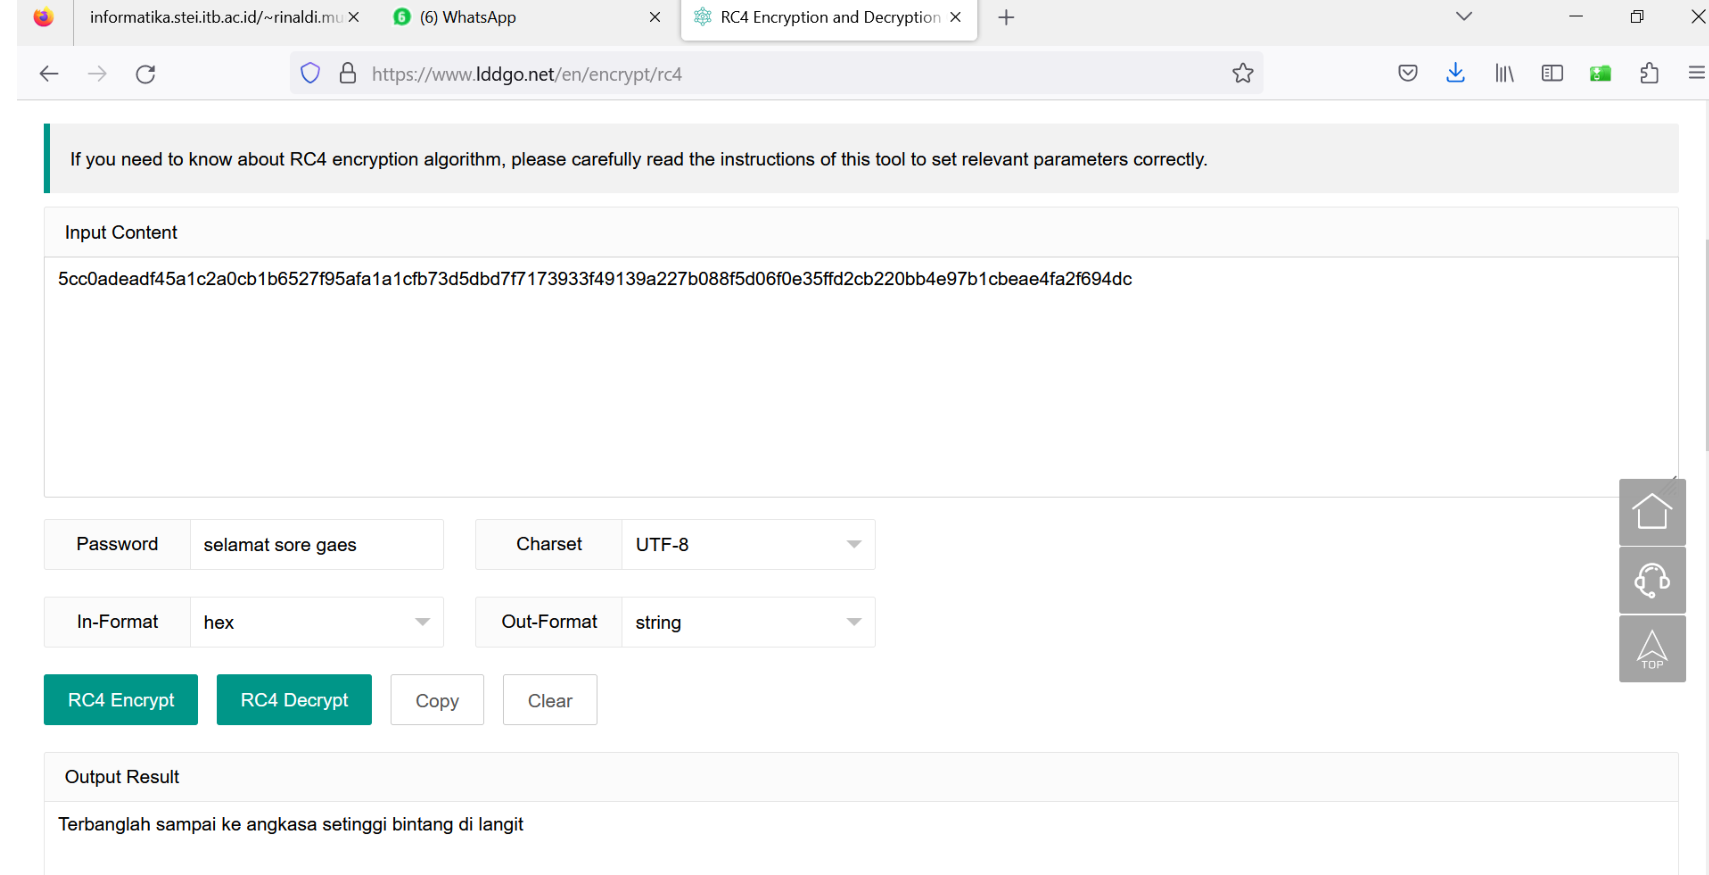
\includegraphics[width=186.90mm,height=240.57mm]{images/llm/page_058_img_01.png}%
\end{textblock*}

\newpage

% --- unit llm 59 ---
% === Halaman 59 (llm) ===

\section*{Library Crypto.Cipher}

\begin{itemize}
    \item Pustaka \texttt{Crypto.Cipher} adalah \textbf{package cipher} di dalam Python.
    \url{https://www.pycrypto.org/api/2.6/Crypto.Cipher-module.html}
    \item Di dalamnya terdapat beberapa modul beberapa cipher, salah satunya RC4 dengan nama modul \texttt{Crypto.Cipher.ARC4}
    \item Cara memanggil Pustaka \texttt{Crypto.Cipher}
    \begin{center}
        \texttt{>> from Crypto.Cipher import ARC4}
    \end{center}
    dengan asumsi sudah meng-install \textit{pycryptodome} dengan menggunakan perintah \texttt{pip}:
    \begin{center}
        \texttt{>> pip install pycryptodome}
    \end{center}
    \item Contoh program Python untuk enkripsi pesan teks dengan RC4 pada slide berikut
\end{itemize}

\newpage

% --- unit llm 60 ---
% === Halaman 60 (llm) ===

\section*{Kode Program RC4 (dalam Bahasa Python)}

\begin{verbatim}
from Crypto.Cipher import ARC4
import base64

def RC4_encrypt(plainteks : str, kunci : bytes) -> str:
    cipher = ARC4.new(kunci)
    cipherteks = cipher.encrypt(plainteks.encode())
    return base64.b64encode(cipherteks).decode()

def RC4_decrypt(cipherteks : str, kunci : bytes) -> str:
    cipher = ARC4.new(kunci)
    cipherteks_decoded = base64.b64decode(cipherteks)
    return cipher.decrypt(cipherteks_decoded)

pesan = input("Ketikkan pesan rahasia:")
kunci = input("Ketikkan kata kunci: ")
kunci = bytearray(kunci, 'utf-8')
ciphertext = RC4_encrypt(pesan, kunci)
print(f"Cipherteks: {ciphertext}")
plaintext = RC4_decrypt(ciphertext, kunci)
print(f"Plainteks semula: {plaintext}")
\end{verbatim}

\newpage

% --- unit llm 61 ---
% === Halaman 61 (llm) ===

\section*{Latihan}

\begin{itemize}
    \item Ubahlah program di atas sehingga dapat digunakan untuk enkripsi dan dekripsi file sembarang
\end{itemize}

\newpage

% --- unit llm 62 ---
% === Halaman 62 (llm) ===

\section*{2. A5}

\begin{itemize}
    \item $A5$ adalah \textit{cipher} alir yang digunakan untuk mengenkripsi transmisi sinyal percakapan dari standard sinyal telepon seluler $GSM$ (\textit{Group Special Mobile}).
    \item Sinyal $GSM$ dikirim sebagai barisan \textit{frame}. Satu \textit{frame} panjangnya $228$ bit dan dikirim setiap $4,6$ milidetik.
    \item $A5$ menghasilkan kunci-alir (\textit{keystream}) sepanjang $228$-bit yang kemudian bit-bitnya di-XOR-kan dengan bit-bit \textit{frame} pesan sepanjang $228$ bit. Kunci eksternal (\textit{session key}) panjangnya $64$ bit.
\end{itemize}

\newpage

% --- unit llm 63 ---
% === Halaman 63 (llm) ===

\begin{itemize}
    \item GSM merupakan standard telepon seluler Eropa. A5 dikembangkan oleh Perancis
    \item Tidak semua operator GSM mengimplementasikan enkripsi, bergantung regulasi (seperti di Indonesia)
    \item A5 ada dua versi:
    \begin{enumerate}
        \item A5/1 : versi kuat A5, digunakan di Eropa
        \item A5/2 (Kasumi) : versi ekspor, lebih lemah
    \end{enumerate}
    \item Algoritma A5/1 pada awalnya rahasia, tetapi pada tahun 1994 melalui \textit{reverse engineering}, algoritmanya terbongkar.
\end{itemize}

\newpage

% --- unit llm 64 ---
% === Halaman 64 (llm) ===

\begin{itemize}
    \item A5 terdiri dari 3 buah $LFSR$, masing-masing panjangnya 19, 22, dan 23 bit (total $= 19 + 22 + 23 = 64$).
    \item Bit-bit di dalam register diindeks dimana bit paling tidak penting (LSB) diindeks dengan 0 (elemen paling kanan).
    \item Luaran (output) dari A5 adalah hasil XOR dari ketiga buah $LFSR$ ini.
    \item A5 menggunakan tiga buah kendali detak (clock) yang variabel:
    \begin{itemize}
        \item Bit ke-8 pada register 1. Bit-bit detak pada bit 13, 16, 17, dan 18
        \item Bit ke-10 pada register 2. Bit-bit detaknya adalah pada bit 20 dan 21
        \item Bit ke-10 pada register 3. Bit-bit detaknya adalah pada bit 7, 20, 21, dan 22
    \end{itemize}
\end{itemize}

\newpage

% --- unit llm 65 ---
% === Halaman 65 (llm) ===

% (tidak ada teks dari model)

% deskripsi: Diagram logika sirkuit digital yang menunjukkan tiga register pergeseran (R1, R2, R3) dengan beberapa tap (titik pengambilan data) yang dihubungkan melalui gerbang XOR untuk menghasilkan urutan bit.
% bbox normalisasi: [0.1380, 0.1830, 0.8310, 0.8230]
\begin{textblock*}{145.53mm}(28.98mm,54.35mm)
\noindent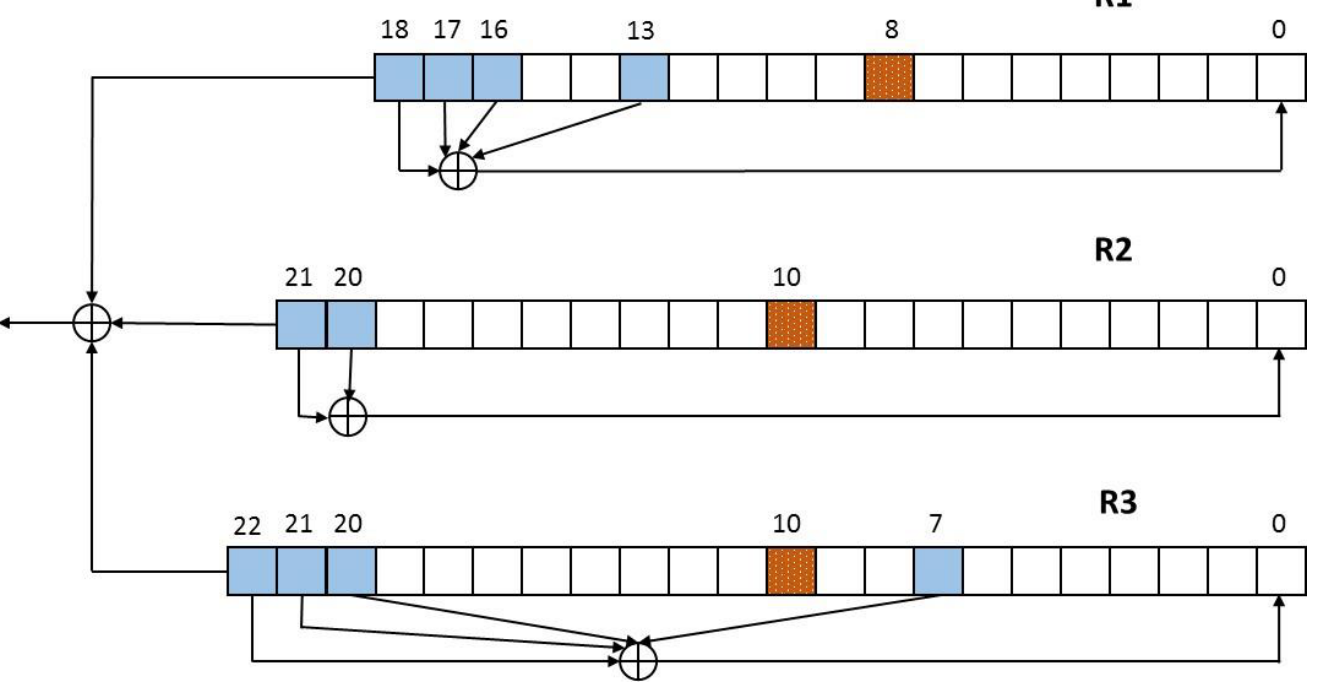
\includegraphics[width=145.53mm,height=190.08mm]{images/llm/page_065_img_01.png}%
\end{textblock*}

\newpage

% --- unit llm 66 ---
% === Halaman 66 (llm) ===

\begin{itemize}
    \item Setiap register didetak dalam fase $stop/go$ dengan menggunakan kaidah mayoritas:
    
    \textcolor{red}{"Pada setiap putaran ($i=1..64$), bit-bit tengah setiap register diperiksa dan bit mayoritasnya ($50\% + 1$) ditentukan. Jika bit tengah sebuah register sama dengan bit mayoritas, maka register tersebut didetak"}
    
    \item Biasanya pada setiap putaran dua atau tiga buah register didetak. Peluang sebuah register didetak pada setiap putaran adalah $\frac{3}{4}$.
    
    \item Ketika sebuah register didetak, semua bit detaknya di-XOR-kan dan hasilnya diletakkan pada posisi LSB (posisi ke-0) dengan mekanisme pergeseran bit-bit ke kiri.
    
    \item Bit paling kiri (MSB) terlempar keluar. Bit yang terlempar dari setiap register di-XOR-kan bersama, bit inilah yang menjadi luaran dari ketiga buah register tadi.
\end{itemize}

\newpage

% --- unit llm 67 ---
% === Halaman 67 (llm) ===

Proses pembangkitan bit-bit acak di dalam A5/1 berdasarkan kunci sesi $K$ adalah sebagai berikut:

\begin{enumerate}
    \item Ketiga register pada awalnya diinisialisasi seluruh bitnya dengan 0. Selanjutnya dilakukan 64 putaran pertama, yaitu 64 bit kunci sesi $K$ dicampur dengan bit register berdasarkan skema berikut:
    
    Pada putaran $0 \le i < 64$,
    \begin{itemize}
        \item bit $K[i]$ ditambahkan ke bit $LSB$ dari setiap register $R$ dengan menggunakan operasi XOR:
        \[ R[0] = R[0] \oplus K[i] \]
        \item tiap register kemudian didetak
    \end{itemize}
\end{enumerate}

\newpage

% --- unit llm 68 ---
% === Halaman 68 (llm) ===

2. Selanjutnya, ketiga register didetak selama 22 putaran tambahan. Selama 22 putaran tersebut, 22-bit dari nomor $frame$ ($F_n$) dicampur dengan bit register berdasarkan skema berikut:

Pada putaran $0 \le i < 22$,

\begin{itemize}
    \item bit $F_n[i]$ ditambahkan ke bit $LSB$ dari setiap register $R$ dengan menggunakan operasi XOR:
    \[ R[0] = R[0] \oplus F_n[i] \]
    \item tiap register kemudian didetak
\end{itemize}

Isi register pada akhir putaran menyatakan kondisi awal untuk pembangkitan $frame$ sepanjang 228-bit.

\newpage

% --- unit llm 69 ---
% === Halaman 69 (llm) ===

\begin{enumerate}
  \item[3.] Ketiga register didetak selama 100 putaran dalam fase $stop/go$ dengan menggunakan kaidah mayoritas, namun bit-bit luarannya dibuang (tidak dipakai).
  \item[4.] Selanjutnya, ketiga register didetak selama 228 putaran dalam fase $stop/go$ menggunakan kaidah mayoritas untuk menghasilkan bit-bit kunci-alir sepanjang 228 bit.
\end{enumerate}

Pada setiap putaran dihasilkan 1 bit yang merupakan hasil peng-XOR-an bit-bit MSB yang terlempar. Total bit luaran adalah 228 bit. Kunci-alir 228-bit inilah yang kemudian digunakan untuk mengenkripsi $frame$ pesan sepanjang 228 bit.

\newpage

% --- unit llm 70 ---
% === Halaman 70 (llm) ===

\begin{itemize}
    \item Algoritma A5/1 telah digunakan untuk mengenkripsi semua percakapan dan komunikasi data melalui telepon seluler GSM di Eropa.
    \item Program A5/1 ditanam di dalam \textit{chip} pada kartu \textit{Simcard}.
    \item Di negara-negara di mana operator telepon seluler dilarang melakukan enkripsi percakapan, seperti di Indonesia, maka program algoritma A5 tidak diaktifkan (\textit{disabled}), sehingga semua sinyal terkirim dalam bentuk plainteks.
\end{itemize}

\newpage

% --- unit llm 71 ---
% === Halaman 71 (llm) ===

\section*{Keamanan A5}

\begin{itemize}
    \item Keamanan A5/1 terletak pada pembangkitan bit-bit acak yang dihasilkan oleh tiga buah LFSR di atas.
    \item Tujuan kriptanalisis A5/1 adalah untuk menemukan kunci sesi yang digunakan dalam pembangkitan bit-bit acak.
    \item Dalam serangan tersebut diasumsikan penyerang mengetahui luaran A5/1 pada periode awal komunikasi, untuk selanjutnya menemukan kunci sesi yang digunakan untuk mendekripsi sisa komunikasi selanjutnya.
\end{itemize}

\newpage

% --- unit llm 72 ---
% === Halaman 72 (llm) ===

\begin{itemize}
  \item Serangan yang dilakukan terhadap A5/1 adalah \textit{known-plaintext attack}.
  \item Serangan semacam ini pertama kali dilakukan oleh Ross Anderson pada tahun 1994.
  \item Ross Anderson mencoba menerka 42 bit isi register R1 dan R2, dan menurunkan 23 bit R3 dari 42 bit tersebut. Pekerjaan menemukan kunci tersebut dilakukan pada komputer PC dan membutuhkan waktu komputasi lebih dari sebulan.
  \item Pada tahun-tahun selanjutnya, para kriptanalis berhasil menemukan kunci hanya dalam waktu beberapa menit saja.
  \item Secara umum, A5/1 sudah berhasil dikriptanalisis.
\end{itemize}

\newpage

% --- unit llm 73 ---
% === Halaman 73 (llm) ===

\vspace{246.51mm}

Interactive Online Simulation of the A5/1 Cipher (\href{https://733amir.github.io/a51-cipher-simulator/}{https://733amir.github.io/a51-cipher-simulator/})

\vspace{10mm}

% deskripsi: Screenshot simulator cipher A5/1 yang menunjukkan input kunci 64-bit, status registrasi, dan diagram aliran register geser (LFSR) yang menghasilkan keystream.
% bbox normalisasi: [0.0300, 0.1100, 0.8400, 0.9400]
\begin{textblock*}{170.10mm}(6.30mm,32.67mm)
\noindent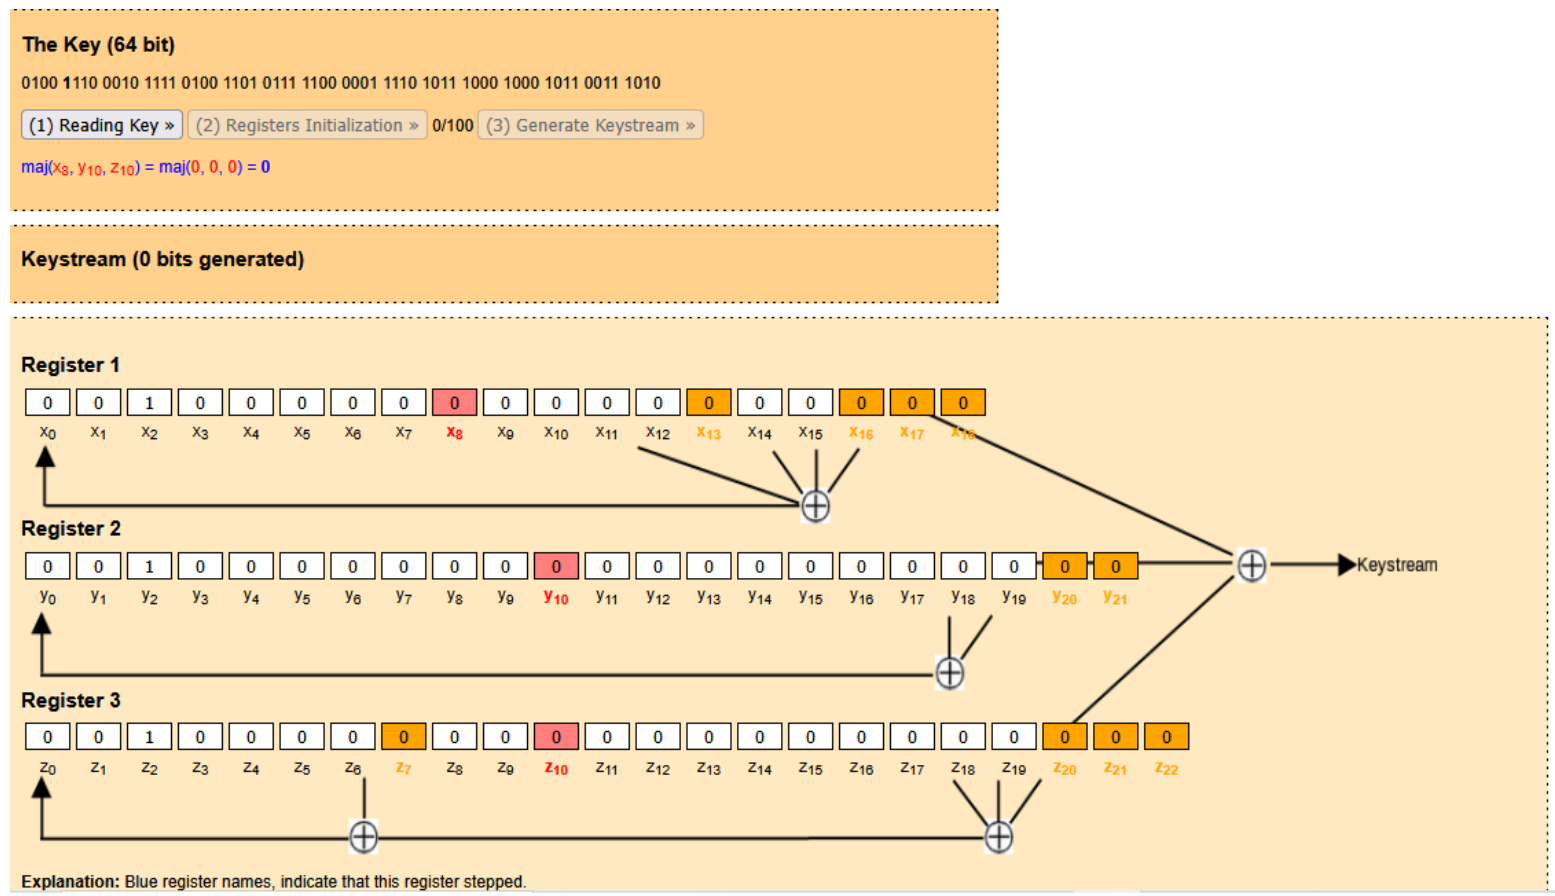
\includegraphics[width=170.10mm,height=246.51mm]{images/llm/page_073_img_01.png}%
\end{textblock*}

\newpage

% --- unit llm 74 ---
% === Halaman 74 (llm) ===

\section*{3. Trivium}

\begin{itemize}
    \item Trivium adalah \textit{cipher-alir} modern, merupakan salah satu \textit{cipher} alir yang di-submit pada kompetisi \textit{stream cipher} eSTREAM pada tahun 2004 -- 2008.
    \item Dibuat oleh Christophe De Cannière dan Bart Preneel.
    \item Menggunakan tiga buah \textit{nonlinear LFSRs} (NLFSR) dengan panjang masing-masing 93, 84, dan 111 bit.
    \item Melakukan XOR terhadap tiga buah luaran NLFSR untuk membangkitkan bit kunci-alir.
    \item Minimalis jika diimplementasikan pada \textit{hardware}:
    \begin{itemize}
        \item total sel register: 288
        \item tiga buah gerbang AND
        \item tujuh buah gerbang XOR
    \end{itemize}
\end{itemize}

\newpage

% --- unit llm 75 ---
% === Halaman 75 (llm) ===

\vspace{100.98mm}

\begin{tabular}{|l|c|c|c|}
\hline
Register length & Feedback bit & Feedforward bit & AND inputs \\ \hline
 A & 93 & 69 & 66 & 91, 92 \\ \hline
 B & 84 & 78 & 69 & 82, 83 \\ \hline
 C & 111 & 87 & 66 & 109, 110 \\ \hline
\end{tabular}

% deskripsi: Diagram sirkuit aliran data untuk generator key stream yang terdiri dari tiga register geser (A, B, C) dengan operasi XOR dan gerbang AND sebagai feedback dan feedforward.
% bbox normalisasi: [0.1100, 0.3000, 0.7300, 0.6400]
\begin{textblock*}{130.20mm}(23.10mm,89.10mm)
\noindent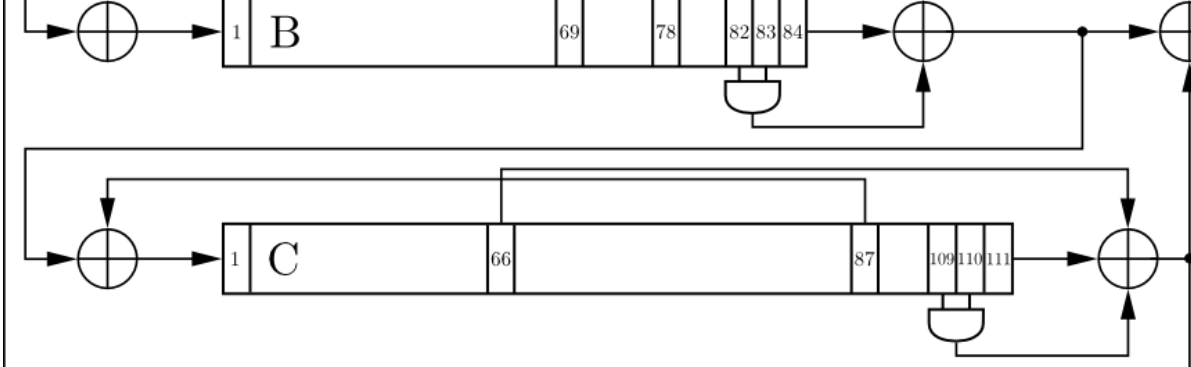
\includegraphics[width=130.20mm,height=100.98mm]{images/llm/page_075_img_01.png}%
\end{textblock*}

\newpage

% --- unit llm 76 ---
% === Halaman 76 (llm) ===

\vspace{60mm}

\textbf{Inisialisasi:}
\begin{itemize}
    \item Masukkan 80-bit \textit{initialization vector} (IV) ke dalam A
    \item Masukkan 80-bit kunci ke dalam B
    \item Set $c_{109}, c_{110}, c_{111} = 1$, sedangkan bit lainnya 0
\end{itemize}

\textbf{Pemanasan (\textit{warming-up}):}
\begin{itemize}
    \item Detak (\textit{clock}) NLFSR $4 \times 288 = 1152$ kali tanpa menghasilkan luaran (luaran diabaikan)
    \item Tujuannya adalah melakukan pencampuran kunci/IV sehingga pengaruh kunci dan IV tersebar ke seluruh register
\end{itemize}

\textbf{Encryption:}
\begin{itemize}
    \item XOR-kan ketiga buah luaran NLFSR untuk membangkitkan kunci-alir $s_i$
    \item XOR-kan $s_i$ dengan bit plainteks $p_i$
\end{itemize}

% deskripsi: Diagram blok arsitektur kriptografi yang menunjukkan tiga register NLFSR (A, B, C) dengan jalur feedback, XOR gates, dan output key stream s_i.
% bbox normalisasi: [0.4800, 0.1000, 0.9300, 0.4400]
\begin{textblock*}{94.50mm}(100.80mm,29.70mm)
\noindent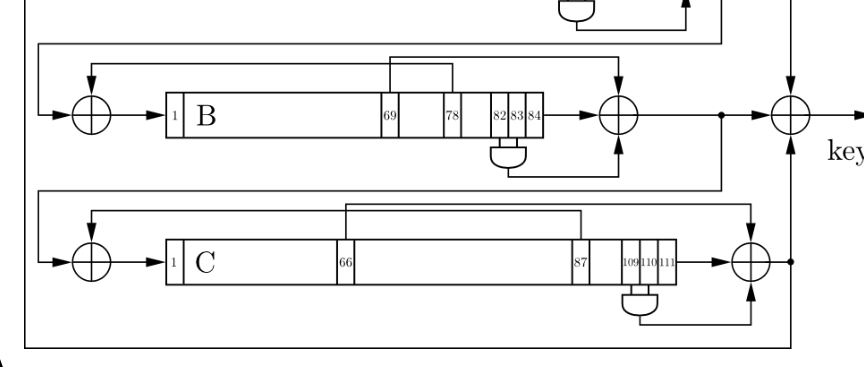
\includegraphics[width=94.50mm,height=100.98mm]{images/llm/page_076_img_01.png}%
\end{textblock*}

\newpage

% --- unit llm 77 ---
% === Halaman 77 (llm) ===

\section*{Kelebihan Trivium}

\begin{enumerate}
    \item Trivium cocok untuk \textit{lightweight cryptography}, karena \textit{state} relatif kecil (hanya 288 bit)
    \item \textit{Hardware efficiency}. Sederhana jika diimplementasikan secara \textit{hardware}, karena struktunta sederhana (terutama terdiri dari \textit{flip-flop/register}, gerbang AND dan OR)
\end{enumerate}

\newpage

% --- unit llm 78 ---
% === Halaman 78 (llm) ===

\section*{4. Salsa20}

\begin{itemize}
    \item Dikembangkan oleh Daniel J. Bernstein pada tahun 2005, merupakan salah satu \textit{cipher} alir yang di-submit pada kompetisi \textit{stream cipher} eSTREAM pada tahun 2004 -- 2008.
    \item Menghasilkan panjang \textit{keystream} 512 bit (atau 64 byte)
    \item Salsa20 menggunakan:
    \begin{itemize}
        \item kunci eksternal dari user (\textit{key}) = 256 bit
        \item nonce (number used once) = 64 bit (ditentukan nilainya oleh aplikasi, harus unik)
        \item counter = 64 bit (dimulai dari 0)
    \end{itemize}
    \item \textit{Nonce} dan \textit{counter} tidak rahasia, \textit{key} harus rahasia
\end{itemize}

\newpage

% --- unit llm 79 ---
% === Halaman 79 (llm) ===

\section*{Daniel J. Bernstein}

\textit{For the American businessman and activist, see Daniel J. Bernstein (businessman).}

\vspace{201.96mm}

\textbf{Daniel Julius Bernstein} (born October 29, 1971) is an American mathematician, cryptologist, and computer scientist. He is a professor of computer science at the University of Illinois Chicago.[2] He was a visiting professor in the department of mathematics and computer science at the Eindhoven University of Technology,[3] and a visiting professor at CASA at Ruhr University Bochum through 2023.[4]

\vspace{20mm}

\subsection*{Early life [ edit ]}

Bernstein attended Bellport High School, a public high school on Long Island, graduating in 1987 at the age of 15.[5] The same year, he ranked fifth in the Westinghouse Science Talent Search.[6] In 1987, he achieved a Top 10 ranking in the William Lowell Putnam Mathematical Competition,[7] and was a member of the second-place team from Princeton University the following year.[8] Bernstein earned a B.A. in mathematics from New York University (1991) and a Ph.D. in mathematics from the University of California, Berkeley (1995), where he studied under Hendrik Lenstra.[1]

% deskripsi: Infobox Wikipedia yang berisi foto potret Daniel J. Bernstein dan informasi singkat seperti tanggal lahir dan tempat lahir.
% bbox normalisasi: [0.5900, 0.2600, 0.8200, 0.9400]
\begin{textblock*}{48.30mm}(123.90mm,77.22mm)
\noindent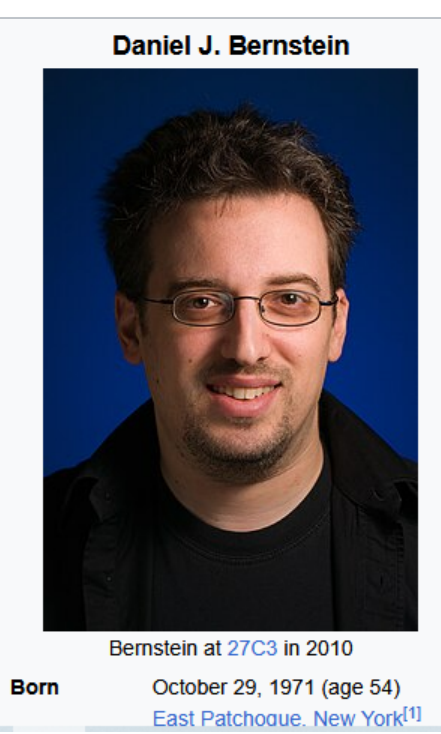
\includegraphics[width=48.30mm,height=201.96mm]{images/llm/page_079_img_01.png}%
\end{textblock*}

\newpage

% --- unit llm 80 ---
% === Halaman 80 (llm) ===

\begin{center}
\Large \textbf{The Salsa20 family of stream ciphers}
\vspace{1cm}
\large Daniel J. Bernstein *
\small Department of Mathematics, Statistics, and Computer Science (M/C 249)\
The University of Illinois at Chicago\
Chicago, IL 60607-7045\
\texttt{snuffle66@box.cr.yp.to}
\end{center}

\noindent \textbf{Abstract.} Salsa20 is a family of 256-bit stream ciphers designed in 2005 and submitted to eSTREAM, the ECRYPT Stream Cipher Project. Salsa20 has progressed to the third round of eSTREAM without any changes. The 20-round stream cipher Salsa20/20 is consistently faster than AES and is recommended by the designer for typical cryptographic applications. The reduced-round ciphers Salsa20/12 and Salsa20/8 are among the fastest 256-bit stream ciphers available and are recommended for applications where speed is more important than confidence. The fastest known attacks use $\approx 2^{153}$ simple operations against Salsa20/7, $\approx 2^{249}$ simple operations against Salsa20/8, and $\approx 2^{255}$ simple operations against Salsa20/9, Salsa20/10, etc. In this paper, the Salsa20 designer presents Salsa20 and discusses the decisions made in the Salsa20 design.

\section{Introduction}

A sender and receiver share a short secret key. They use the secret key to encrypt a series of messages. A message could be short, just a few bytes, but it could be

\newpage

% --- unit llm 81 ---
% === Halaman 81 (llm) ===

\textbf{Step 1:} Tentukan parameter masukan (key, nonce, counter)

\textbf{Step 2:} Inisialisasi matriks \textit{state} berukuran $4 \times 4$, setiap elemen matriks berukuran 1 word, 1 word = 32 bit. Total ukuran matriks $16 \times 32 \text{ bit} = 512 \text{ bit}$. \textit{State} berisi konstanta ('expand 32-byte k'), \textit{key}, \textit{counter}, dan \textit{nonce} dengan pengaturan letak sebagai berikut:

\vspace{10mm}

\textbf{Catatan:} Di dalam kdoe program, matriks \textit{state} dinyatakan sebagai sebuah larik $\text{in}[0..15]$

% deskripsi: Diagram matriks state Salsa20 yang menunjukkan indeks elemen (0-15) dan pemetaan tata letak konstanta, key, nonce, dan posisi (counter) dalam matriks 4x4.
% bbox normalisasi: [0.1060, 0.4250, 0.6950, 0.8550]
\begin{textblock*}{123.69mm}(22.26mm,126.22mm)
\noindent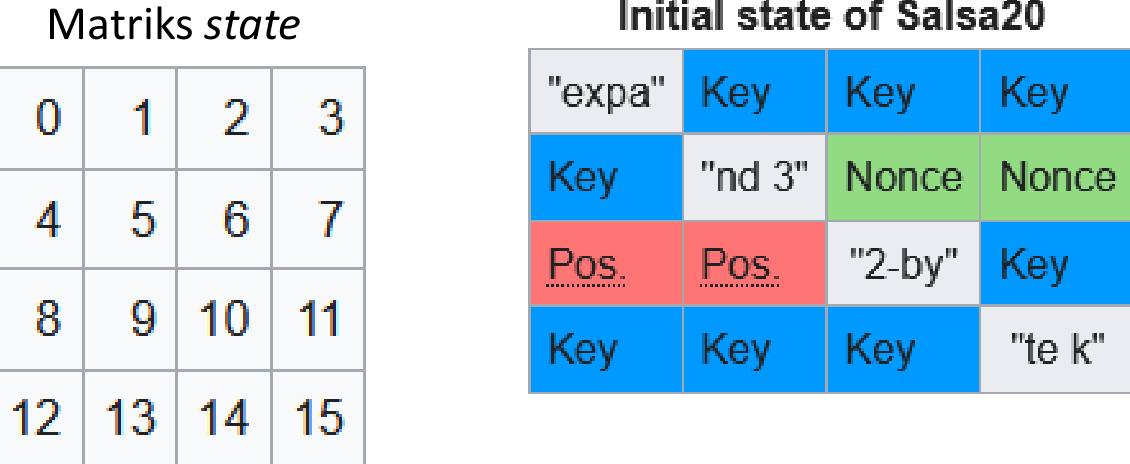
\includegraphics[width=123.69mm,height=127.71mm]{images/llm/page_081_img_01.png}%
\end{textblock*}

\newpage

% --- unit llm 82 ---
% === Halaman 82 (llm) ===

\textbf{Step 3:} Simpan salinan state awal ke dalam larik x

\begin{verbatim}
for (i = 0; i < 16; ++i)
    x[i] = in[i];
\end{verbatim}

\textbf{Step 4:} Lakukan 20 putaran (= 10 putaran ganda), satu putaran ganda terdiri dari 10 \textit{column round} dan 10 \textit{row round}.

Double-round 1
$\rightarrow$ Column Round
$\rightarrow$ Row Round

Double-round 2
$\rightarrow$ Column Round
$\rightarrow$ Row Round

$\dots$

Double-round 10
$\rightarrow$ Column Round
$\rightarrow$ Row Round

\newpage

% --- unit llm 83 ---
% === Halaman 83 (llm) ===

\begin{itemize}
  \item \textit{Column round} dan \textit{row round} dilakukan di dalam sebuah struktur \textit{quarter round} $\text{QR}(a, b, c, d)$ yang menerima empat \textit{word} sebagai masukan dan menghasilkan empat word luaran:
  
  \begin{align*}
    b & \gets b \oplus (a + d) \lll 7; \\
    c & \gets c \oplus (b + a) \lll 9; \\
    d & \gets d \oplus (c + b) \lll 13; \\
    a & \gets a \oplus (d + c) \lll 18;
  \end{align*}
  
  $\lll k$ adalah pergeseran bit ke kiri sejauh $k$ bit dan bersifat rotasi (siklik)\
  $+$ adalah penjumlahan bit dalam $\bmod 2^{32}$
\end{itemize}

\vspace{20mm}

\textbf{Quarter Round merupakan inti Salsa20}

% deskripsi: Diagram alur operasi Quarter Round yang menunjukkan transformasi variabel a, b, c, dan d menggunakan operasi penjumlahan, rotasi bit (<<<), dan XOR.
% bbox normalisasi: [0.6020, 0.2240, 0.8240, 0.9370]
\begin{textblock*}{46.62mm}(126.42mm,66.53mm)
\noindent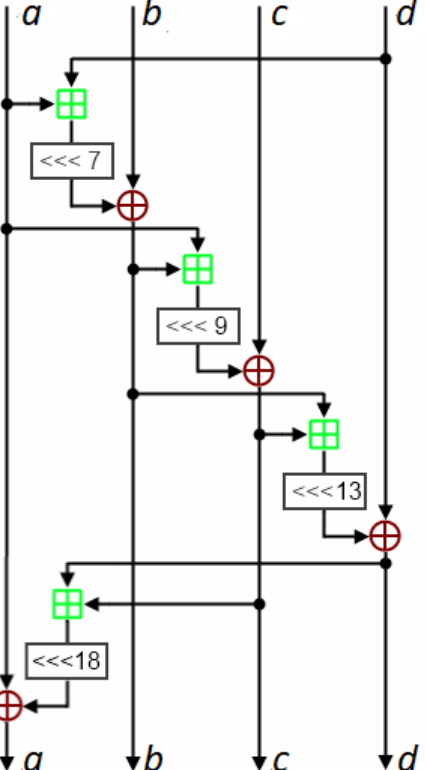
\includegraphics[width=46.62mm,height=211.76mm]{images/llm/page_083_img_01.png}%
\end{textblock*}

\newpage

% --- unit llm 84 ---
% === Halaman 84 (llm) ===

\begin{itemize}
  \item \textit{Column round} menerapkan $\text{QR}(a, b, c, d)$ kepada tiap kolom matriks $\text{state } 4\times 4$, sedangkan \textit{row round} menerapkannya kepada tiap baris matriks.
\end{itemize}

\vspace{53.46mm}

\noindent // Column round
\[
\begin{aligned}
\text{QR}(0, 4, 8, 12) & \quad // \text{ kolom 1} \\
\text{QR}(5, 9, 13, 1) & \quad // \text{ kolom 2} \\
\text{QR}(10, 14, 2, 6) & \quad // \text{ kolom 3} \\
\text{QR}(15, 3, 7, 11) & \quad // \text{ kolom 4}
\end{aligned}
\]

\vspace{10mm}

\noindent // Row round
\[
\begin{aligned}
\text{QR}(0, 1, 2, 3) & \quad // \text{ baris 1} \\
\text{QR}(5, 6, 7, 4) & \quad // \text{ baris 2} \\
\text{QR}(10, 11, 8, 9) & \quad // \text{ baris 3} \\
\text{QR}(15, 12, 13, 14) & \quad // \text{ baris 4}
\end{aligned}
\]

% deskripsi: Matriks state 4x4 yang berisi angka 0 sampai 15
% bbox normalisasi: [0.7500, 0.2600, 0.9100, 0.5500]
\begin{textblock*}{33.60mm}(157.50mm,77.22mm)
\noindent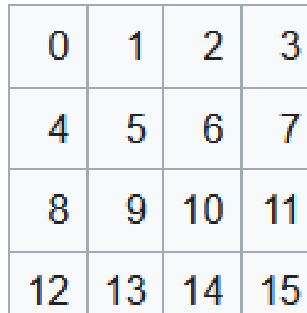
\includegraphics[width=33.60mm,height=86.13mm]{images/llm/page_084_img_01.png}%
\end{textblock*}

% deskripsi: Definisi algoritma QR(a, b, c, d) dengan operasi XOR dan rotasi
% bbox normalisasi: [0.4700, 0.2800, 0.7000, 0.4600]
\begin{textblock*}{48.30mm}(98.70mm,83.16mm)
\noindent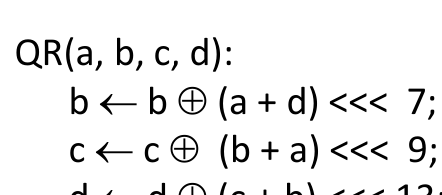
\includegraphics[width=48.30mm,height=53.46mm]{images/llm/page_084_img_02.png}%
\end{textblock*}

% deskripsi: Implementasi C++ makro untuk ROTL dan QR
% bbox normalisasi: [0.4700, 0.6500, 0.8100, 0.9200]
\begin{textblock*}{71.40mm}(98.70mm,193.05mm)
\noindent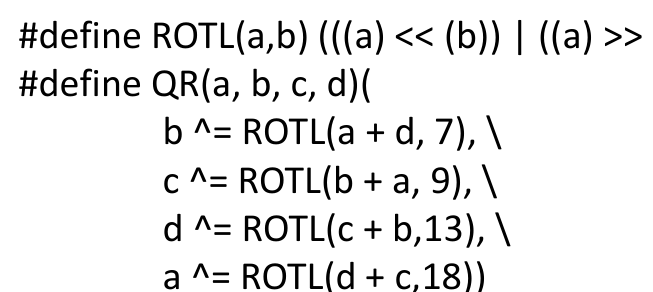
\includegraphics[width=71.40mm,height=80.19mm]{images/llm/page_084_img_03.png}%
\end{textblock*}

\newpage

% --- unit llm 85 ---
% === Halaman 85 (llm) ===

\textbf{Step 5:} State hasil 10 putaran-ganda dijumlahkan dengan state awal yang disimpan pada step 3:

\[
\mathbf{y = (x' + x) \pmod{2^{32}}}
\]

Jika plainteks berukuran n x 512 bit, maka Salsa20 dieksekusi sebanyak n kali, dengan \textit{counter} bertambah 1, sedangkan \textit{nonce} tetap.

\textbf{Kode program C++:}

\begin{verbatim}
#include <stdint.h>
#define ROTL(a,b) (((a) << ((b)) | ((a) >> (32 - (b)))))
#define QR(a, b, c, d)(\ 
    b ^= ROTL(a + d, 7), \ 
    c ^= ROTL(b + a, 9), \ 
    d ^= ROTL(c + b, 13), \ 
    a ^= ROTL(d + c, 18))
#define ROUNDS 20
\end{verbatim}

\newpage

% --- unit llm 86 ---
% === Halaman 86 (llm) ===

\begin{verbatim}
void salsa20_block(uint32_t out[16], uint32_t const in[16])
{
    int i;
    uint32_t x[16];

    for (i = 0; i < 16; ++i)
        x[i] = in[i];
    // 10 loops x 2 rounds/loop = 20 rounds
    for (i = 0; i < ROUNDS; i += 2) {
        // Column round
        QR(x[0], x[4], x[8], x[12]); // column 1
        QR(x[5], x[9], x[13], x[1]); // column 2
        QR(x[10], x[14], x[2], x[6]); // column 3
        QR(x[15], x[3], x[7], x[11]); // column 4
        // Row round
        QR(x[0], x[1], x[2], x[3]); // row 1
        QR(x[5], x[6], x[7], x[4]); // row 2
        QR(x[10], x[11], x[8], x[9]); // row 3
        QR(x[15], x[12], x[13], x[14]); // row 4
    }
    for (i = 0; i < 16; ++i)
        out[i] = x[i] + in[i];
}
\end{verbatim}

\begin{flushright}
Sumber: Wikipedia
\end{flushright}

\newpage

% --- unit llm 87 ---
% === Halaman 87 (llm) ===

\section*{Kelebihan Salsa20}

\begin{enumerate}
    \item \textbf{Sangat cepat}\
    Salsa20 hanya menggunakan operasi yang sangat sederhana (AXR):
    \begin{itemize}
        \item penjumlahan (\textit{add}) modulo $2^{32}$,
        \item XOR,
        \item rotasi bit.
    \end{itemize}

    \item \textbf{Memiliki keamanan yang baik}\
    Salsa20 dirancang dengan 20 putaran untuk memberikan difusi yang kuat. Maksudnya, perubahan kecil pada \textit{key, nonce, counter}, akan menghasilkan perubahan yang besar pada keystream.
\end{enumerate}

\newpage

% --- unit llm 88 ---
% === Halaman 88 (llm) ===

\textbf{3. Cocok untuk perangkat dengan sumber daya terbatas}\\ Karena operasi internalnya sederhana, Salsa20 dapat diimplementasikan dengan baik pada berbagai perangkat, termasuk perangkat yang kemampuan komputasinya terbatas.\\
\vspace{5mm}
\textbf{4. Cocok untuk implementasi perangkat lunak}\\ Salsa20 dapat memperoleh performa yang baik hanya dengan operasi integer dasar. Karena itu Salsa20 sangat populer dalam komunitas kriptografi, dan desainnya kemudian menjadi dasar bagi \textbf{ChaCha}, yang akhirnya lebih banyak digunakan dalam protokol modern.\\
\vspace{5mm}
\textbf{5. Menghasilkan blok \textit{keystream} yang besar}\\ Satu blok Salsa20 menghasilkan $16 \times 32 \text{ bit} = 512 \text{ bit} = 64 \text{ byte keystream}$. Jika plaintext panjang, counter tinggal dinaikkan untuk menghasilkan blok berikutnya.

\newpage

% --- unit llm 89 ---
% === Halaman 89 (llm) ===

\textbf{6. \textit{Keystream} dapat dihasilkan secara paralel}

Salah satu karakteristik penting Salsa20 adalah setiap blok \textit{keystream} bergantung pada \textit{key}, \textit{nonce}, dan \textit{counter}.

Secara konseptual:

\begin{align*}
\text{Key + Nonce + Counter 0} & \rightarrow \text{Keystream 0} \\
\text{Key + Nonce + Counter 1} & \rightarrow \text{Keystream 1} \\
\text{Key + Nonce + Counter 2} & \rightarrow \text{Keystream 2} \\
\text{Key + Nonce + Counter 3} & \rightarrow \text{Keystream 3}
\end{align*}

Blok-blok tersebut pada prinsipnya dapat dihitung secara independen. Ini berbeda dari beberapa konstruksi \textit{stream cipher} yang memiliki ketergantungan berantai antar keystream.

\newpage

% --- unit llm 90 ---
% === Halaman 90 (llm) ===

\section*{ChaCha20}

\begin{itemize}
    \item ChaCha20 merupakan modifikasi dari Salsa20 yang dipublikasikan oleh Bernstein pada tahun 2008. ChaCha20 merupakan keluarga ChaCha (ChaCha lainnya: Chacha6, ChaCha7)
    \item Alasannya terutama adalah untuk memperoleh difusi yang lebih baik pada struktur internal sekaligus mempertahankan kecepatan dan kesederhanaan desain ARX (add, rotate, xor).
    \item ChaCha20 Mempertahankan keamanan Salsa20 sambil memperbaiki karakteristik desain
    \item Salah satu tujuan penting desain ChaCha adalah memperoleh implementasi yang sangat efisien pada perangkat lunak.
    \item ChaCha20 menjadi sangat populer dalam protokol modern
\end{itemize}

\newpage

% --- unit llm 91 ---
% === Halaman 91 (llm) ===

\vspace{280.37mm}

Perbedaan ChaCha dengan Salsa:

\vspace{76.63mm}

1. Initial state

\vspace{40mm}

2. Quarter round QR

\begin{align*}
a &\leftarrow a + b; \quad d \leftarrow d \oplus a; \quad d \leftarrow d \lll 16; \\
c &\leftarrow c + d; \quad b \leftarrow b \oplus c; \quad b \leftarrow b \lll 12; \\
a &\leftarrow a + b; \quad d \leftarrow d \oplus a; \quad d \leftarrow d \lll 8; \\
c &\leftarrow c + d; \quad b \leftarrow b \oplus c; \quad b \leftarrow b \lll 7;
\end{align*}

% deskripsi: Tabel initial state of ChaCha yang terdiri dari konstanta, key, counter, dan nonce.
% bbox normalisasi: [0.1070, 0.1760, 0.4080, 0.4340]
\begin{textblock*}{63.21mm}(22.47mm,52.27mm)
\noindent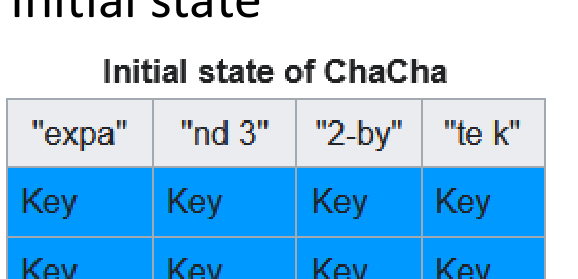
\includegraphics[width=63.21mm,height=76.63mm]{images/llm/page_091_img_01.png}%
\end{textblock*}

% deskripsi: Diagram alir operasi Quarter Round (QR) pada ChaCha dengan simbol penjumlahan, XOR, dan rotasi bit.
% bbox normalisasi: [0.5810, 0.0000, 0.9720, 0.9440]
\begin{textblock*}{82.11mm}(122.01mm,0.00mm)
\noindent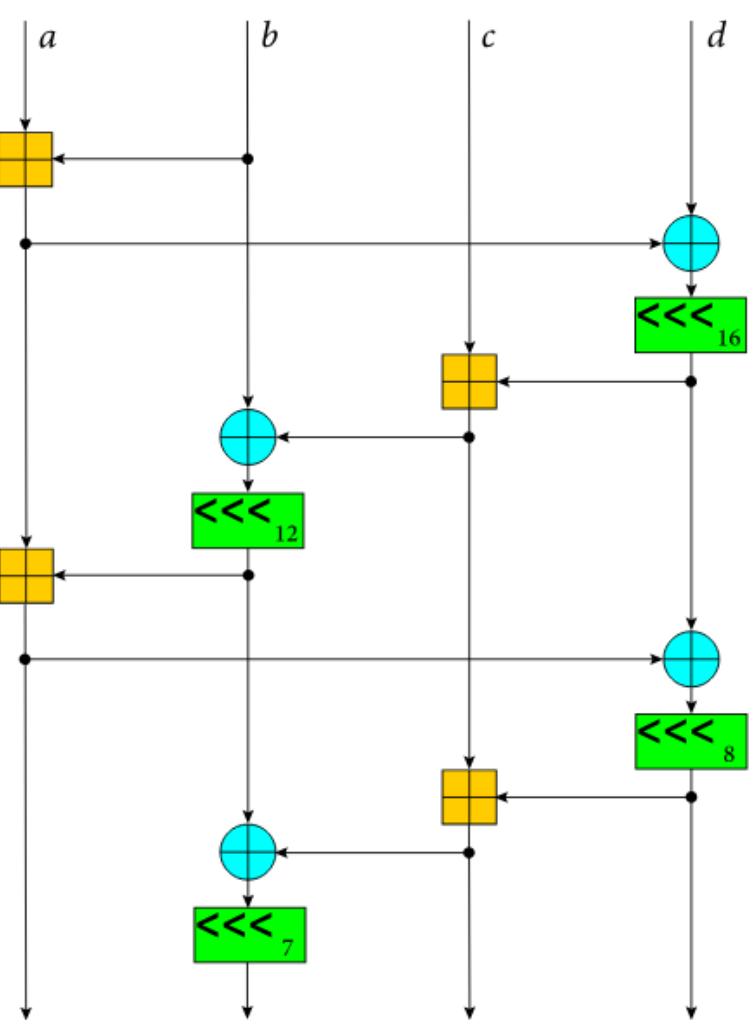
\includegraphics[width=82.11mm,height=280.37mm]{images/llm/page_091_img_02.png}%
\end{textblock*}

\newpage

% --- unit llm 92 ---
% === Halaman 92 (llm) ===

3. Column round dan diagonal round

// Column round

\vspace{99.20mm}

\begin{align*}
QR(0, 4, 8, 12) & \quad // \text{ kolom 1} \\
QR(1, 5, 9, 13) & \quad // \text{ kolom 2} \\
QR(2, 6, 10, 14) & \quad // \text{ kolom 3} \\
QR(3, 7, 11, 15) & \quad // \text{ kolom 4}
\end{align*}

\vspace{10mm}

// Diagonal round

\begin{align*}
QR(0, 5, 10, 15) & \quad // \text{ diagonal 1} \\
QR(1, 6, 11, 12) & \quad // \text{ diagonal 2} \\
QR(2, 7, 8, 13) & \quad // \text{ diagonal 3} \\
QR(3, 4, 9, 14) & \quad // \text{ diagonal 4}
\end{align*}

% deskripsi: Tabel 4x4 berisi angka 0 sampai 15 yang menunjukkan indeks posisi elemen untuk proses Column round dan Diagonal round.
% bbox normalisasi: [0.5960, 0.2860, 0.7600, 0.6200]
\begin{textblock*}{34.44mm}(125.16mm,84.94mm)
\noindent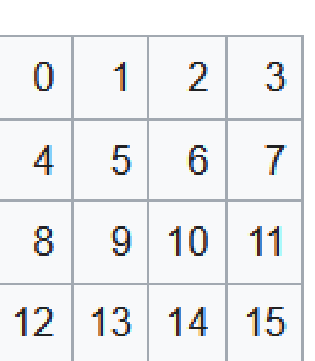
\includegraphics[width=34.44mm,height=99.20mm]{images/llm/page_092_img_01.png}%
\end{textblock*}

\newpage

% --- unit llm 93 ---
% === Halaman 93 (llm) ===

\vspace{279.18mm}

Sumber: Wikipedia

% deskripsi: Implementasi kode program C untuk algoritma ChaCha20, mencakup makro ROTL, makro QR (Quarter Round), dan fungsi chacha\_block.
% bbox normalisasi: [0.0100, 0.0200, 0.9700, 0.9600]
\begin{textblock*}{201.60mm}(2.10mm,5.94mm)
\noindent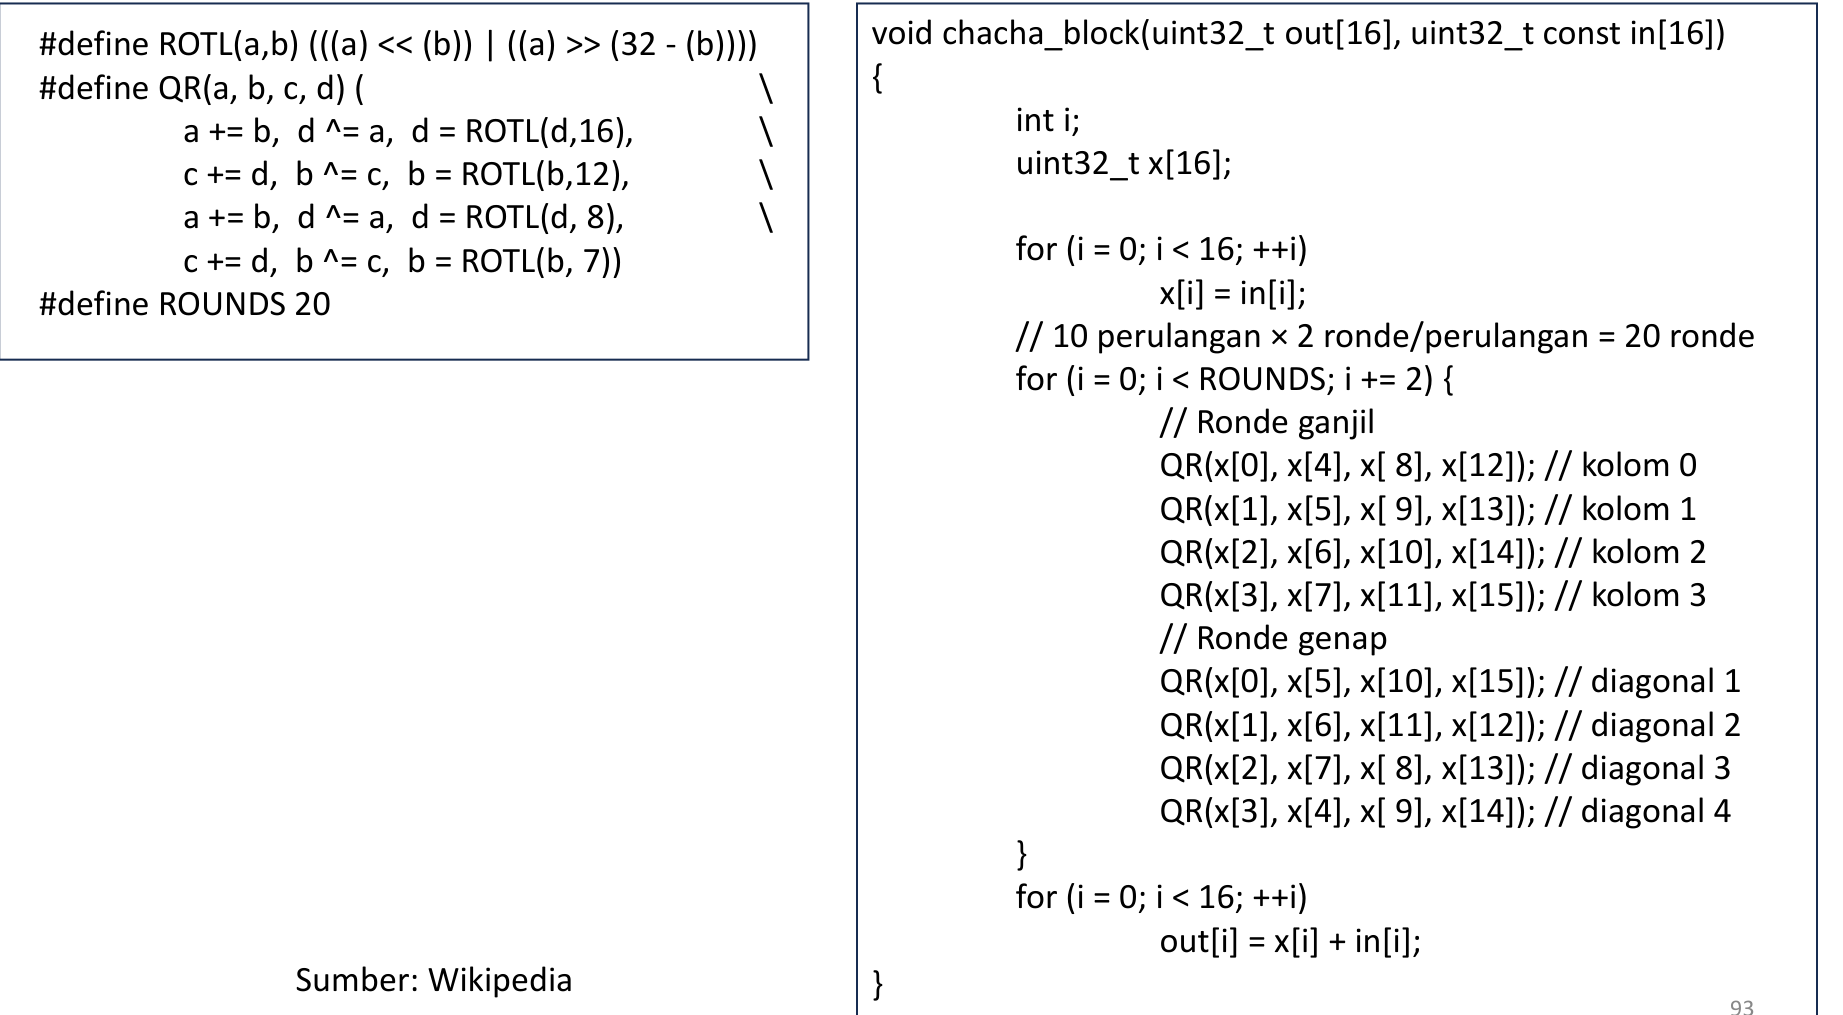
\includegraphics[width=201.60mm,height=279.18mm]{images/llm/page_093_img_01.png}%
\end{textblock*}

\newpage

% --- unit llm 94 ---
% === Halaman 94 (llm) ===

Sekian

\end{document}
